\documentclass[
    BCOR=2cm,
    DIV=14,
    fontsize=12bp,
    footsepline=true,
    headsepline=true,
    listof=numbered,
    twoside=semi,
    version=last,
]{scrbook}

% KOMA Setup
\RedeclareSectionCommand[beforeskip=0pt]{chapter}

% Language Setup
\usepackage{polyglossia}
\setdefaultlanguage[spelling=new,babelshorthands=true]{german}

% Fonts Setup
\usepackage{lmodern}
\usepackage{fontspec}
\setmonofont{Consolas}[LetterSpace=-0.5,Scale=0.75]
\usepackage[
    onehalfspacing,
    nodisplayskipstretch,
]{setspace}
\directlua{
    % luaotfload has a predefined keepligature function at the time of writing.
    % microtype will warn about the function being overwritten, which is not really interesting though.
    luaotfload.letterspace.keepligature = false
}
\usepackage[
    activate={true,nocompatibility}, % Enable Protrusion/Expansion refinements
    babel=true, % Try to use localized informations
    final, % Ignore the global draft option
    tracking=true, % Enable letter spacing refinements
]{microtype}

% Packages that must be loaded before general ones
\usepackage[
    outputdir=build,
]{minted}
\setminted[cpp]{
    baselinestretch=1,
    linenos=true,
}

% General packages
\usepackage{booktabs}
\usepackage{csquotes}
\usepackage{etoolbox}
\usepackage{graphicx}
\usepackage{mathtools}
\usepackage{subcaption}
\usepackage{svg}
\usepackage{tabu}
\usepackage{wrapfig}

% Packages that must be loaded after general ones
\usepackage[
    warnings-off={mathtools-colon,mathtools-overbracket},
]{unicode-math}
\usepackage[
    binary-units=true,
    locale=DE,
]{siunitx}

% Remove vertical space between enumeration items
\usepackage[shortlabels]{enumitem}
\setlist[itemize]{noitemsep}
\setlist[enumerate]{noitemsep}

% hyperref strongly suggests loading it as the last package.
% Only few packages are an exception to this rule. See here:
%   https://tex.stackexchange.com/q/1863
\usepackage{hyperref}
\hypersetup{
    colorlinks=true,
    german,
    pdfauthor={Leonard Hecker},
    unicode=true,
}

% If biblatex is loaded after hyperref, links will be created.
\usepackage[
    backend=biber,
    block=ragged,
    doi=false,
    eprint=false,
    sorting=nyt, % sort by name, year, title
    sortlocale=de_DE,
    style=numeric-comp, % cite using numbers
]{biblatex}
\addbibresource{main.bib}

% Fixes various issues of KOMA-script with other packages.
\usepackage{scrhack}

% HTW Dresden requires 1.25cm of head/foot skip.
\setlength{\headsep}{1.25cm}
\setlength{\skip\footins}{1.25cm}

% \unicodefont will make it possible to render certain uncommon unicode symbols.
\newfontfamily{\unicodefont}{DejaVu Sans}[Scale=MatchLowercase]
\DeclareTextFontCommand{\textunicode}{\unicodefont}

% Disable the old-fashioned addition of extra spacing after the end of a sentence.
\frenchspacing

% Reduce the amount of hyphenations, while allowing far greater leeway when stretching a line.
\tolerance=10000
\hbadness=10000
\hyphenpenalty=4000

% Remove indentation for wrapfigure captions.
\captionsetup{
    subrefformat=parens,
}
\captionsetup[wrapfigure]{
    format=plain,
    subrefformat=parens,
}

% Swap paragraph indentation with a skip.
\setlength{\parindent}{0bp}
\setlength{\parskip}{6bp}

% Reduce tabu's line height by a bit compared to regular text.
\setlength{\tabulinesep}{3bp}

% A hack to make wrapfigure align with the top of the paragraph's first line.
\setlength{\intextsep}{12bp}
\newcommand{\wrapfigurefix}[1]{\setlength{\intextsep}{#1}}
\newcommand{\wrapfigureunfix}{\setlength{\intextsep}{12bp}}


% Translations for listings
\providecommand*{\listingautorefname}{Programmausdruck}
\renewcommand{\listingscaption}{Programmausdruck}

% Some document specific commands
\newcommand{\ditto}{---\raisebox{-0.5ex}{''}---}
\newcommand{\systemfootnote}{\footnote{Linux; \textsc{gcc} 8.3 mit \texttt{-Ofast}; i7--8700k @ \SI{4.2}{\giga\hertz}; DDR4 @ \SI{3.2}{\giga\hertz}, 16--18--18--38}}

\begin{document}

% Some options (like the following) are being set at \begin{document}.
% --> Set them now.
\sloppy
\setlength{\abovedisplayskip}{3bp}
\setlength{\belowdisplayskip}{6bp}
\setlength{\abovedisplayshortskip}{3bp}
\setlength{\belowdisplayshortskip}{6bp}

\frontmatter{}
\begin{titlepage}
    {
        \centering
        \large
        {\scshape Hochschule für Technik und Wirtschaft Dresden \par}
        {\scshape Fakultät Informatik/Mathematik \par}
        \vfill
        {\bfseries\huge Bachelorarbeit \par}
        \vspace{0.5cm}
        {im Studiengang Informatik \par}
        \vspace{1cm}
        {\bfseries\LARGE Vektorisierung von Freihandzeichnungen \par}
        \par
    }
    \vfill
    \begin{tabu}{ll}
        eingereicht von: & Leonard Hecker \\
        eingereicht am:  & 24.04.2019 \\
        Betreuer:        & Prof.\ Dr.\ Georg Freitag \\
                         & Prof.\ Dr.\ Marius Brade
    \end{tabu}
\end{titlepage}

\cleardoublepage{}
\tableofcontents{}


\mainmatter{}
\chapter{Einleitung}

Linienzeichnungen, beziehungsweise Skizzierungen, werden auch heute noch häufig \enquote{analog} auf zum Beispiel Papier, Tafeln oder Whiteboards erstellt.
Die Anwendung Mind-Objects jedoch erlaubt es einem Nutzer dies digital auf einem Mobilgerät zu tun.
Anders als bei üblichen Zeichenprogrammen werden die hierbei gezeichneten Linien aber nicht als Raster-, sondern als Vektorgrafik aufgezeichnet.
Hierdurch wird es dem Nutzer ermöglicht, auch nachträglich noch beliebige Teile der Zeichnung zu skalieren, zu verschieben oder gar zu löschen, wodurch ein hohes Maß an Flexibilität während der Erstellung der Zeichnung erhalten bleibt.
Im Kontrast dazu stehen \enquote{traditionelle} Zeichnungen, in denen derartige, nachträgliche Änderungen nur schwer, oder gar nicht möglich sind.

Bisher mangelt es der Anwendung Mind-Objects jedoch noch an der Fähigkeit eben jene, potentiell bereits existierenden, \enquote{analogen} Zeichnungen als Vektorgrafik importieren zu können, damit sie nahtlos weiterverarbeitet und transformiert werden können.
Hierfür ist es denkbar, dass es dem Nutzer ermöglicht wird, ein Foto mithilfe der Anwendung aufzunehmen, welches daraufhin vektorisiert wird.

Die vorliegende Arbeit beschäftigt sich im Detail mit Methoden zur Vektorisierung solcher Fotografien.
Ziel ist es, eine Programmbibliothek zu entwickeln, welche später in die Mobilanwendung integriert werden kann und den gesamten Prozessablauf von einer Fotografie bis hin zur Vektorgrafik implementiert.
Die hierbei vektorisierten Linien sollen das optische Bild der ursprünglichen Fotografie möglichst getreu widerspiegeln, weshalb es unabdingbar ist, dass die Form und somit die Strichstärke der Linien erhalten bleibt.
Weiterhin ist es wichtig, dass nur so viele Knotenpunkte wie notwendig für die berechneten Linien verwendet werden, damit die Darstellungsgeschwindigkeit der Anwendung nicht negativ beeinflusst wird.
Letztendlich müssen Algorithmen gewählt werden, welche auch bei der Verwendung auf CPUs von Mobilgeräten ausreichend schnell sind.

\chapter{Grundlagen}%
\label{cha:essentials}

\section{Binarisierung}%
\label{sec:essentials_binarization}

Die Binarisierung ist eine Spezialform der sogenannten Segmentierung eines Bildes.
Während bei der allgemeinen Segmentierung das Bild generell in eine beliebige, aber finite, Anzahl von Regionen aufgeteilt wird, bezieht sich die Binarisierung konkret auf die Partitionierung in exakt zwei Teile.
Üblicherweise wird hierbei ein Graustufen- beziehungsweise Schwarzweißbild in ein Binärbild umgewandelt, mit dem Ziel das Bild in Hinter- und Vordergrund beziehungsweise Schwarz und Weiß aufzuteilen.

Die einfachste und am häufigsten verwendete Variante ist das sogenannte \enquote{Schwellenwertverfahren}.
Angenommen folgende Definitionen gelten:

\begin{tabu}{lX}
    \(P(x,y)\) & Graustufenwert an der Stelle \((x,y)\) \\
    \(P'(x,y)\) & Resultierender Binärwert an der Stelle \((x,y)\) \\
    \(T(x,y)\) & Schwellenwert an der Stelle \((x,y)\)
\end{tabu}

Dann ist das \enquote{Schwellenwertverfahren} definiert als:
\begin{gather}
    P'(x,y) = \begin{cases}
        \text{schwarz} & \text{wenn } P(x,y) < T(x,y) \\
        \text{weiß} & \text{ansonsten}
    \end{cases}
\end{gather}

Für die konkrete Schwellenwertfunktion steht eine große Auswahl an Definitionen zur Verfügung~\cite{DBLP:journals/jei/SezginS04}.
Generell lassen sich jedoch die Algorithmen in zwei Arten aufteilen: Globale und Lokale.
Erstere berechnen einen konstanten Schwellenwert \(T(x,y) = k\), welcher \enquote{global} auf die gesamte Grafik angewendet wird.
Letztere hingegen berechnen den Schwellenwert separat für jede Stelle \((x,y)\) anhand von in der \enquote{lokalen} Umgebung vorkommenden Statistiken.

Aufgrund dieser Eigenschaft sind lokale Schwellenwertfunktionen in der Lage, auch bei ungleichmäßiger Ausleuchtung des Bilds zufriedenstellende Ergebnisse zu liefern, da es der Funktion erlaubt wird, sich den lokal ändernden Gegebenheiten des Bilds anzupassen.
Dies erhöht jedoch signifikant den Rechenaufwand, da die Schwelle nicht nur ein einzelnes Mal, sondern für jedes Pixel neu berechnet werden muss.
Ein weiteres Problem ist der Umstand, dass eine passende Größe der \enquote{lokalen Umgebung}, beziehungsweise der Fenstergröße, gewählt werden muss.
Ist die Fenstergröße zu klein, so kann dies die Statistik verfälschen und zu optisch stark inkorrekten Ergebnissen führen.
Ist sie hingegen zu groß so steigt der Rechenaufwand entsprechend signifikant.
Auch die Fähigkeit zur Anpassung an neue Gegebenheiten des Bilds wird hierdurch abgeschwächt.

Globale Schwellenwertfunktionen unterliegen keinen solchen Einschränkungen, weshalb sie in der Regel bei einem geringeren Rechenaufwand bessere Ergebnisse erzielen, sofern die entsprechenden Grafiken keine Binarisierung benötigen, die sich lokalen Gegebenheiten anpassen muss.
Dies ist zum Beispiel in der Regel der Fall für annähernd saubere Aufnahmen von Textdokumenten, welche sich bereits optisch klar in Schwarz und Weiß aufteilen lassen.

\autoref{fig:essentials_binarization_uneven_illumination} zeigt die Vorteile lokaler Schwellenwertfunktionen exemplarisch an ihrer Anpassungsfähigkeit bei ungleichmäßiger Ausleuchtung.
Dem gegenüber steht unter anderem der Nachteil der finiten Fenstergröße in \autoref{fig:essentials_binarization_window_size}.
Da diese in der Abbildung zu Demonstrationszwecken bewusst kleiner als die Breite des Person gewählt wurde, passt sich die Schwellenwertfunktion der dunklen Farbe der Jacke an und senkt die lokal zu erreichende Schwelle.
Hierdurch erscheint der Großteil des Person fälschlicherweise Weiß und nur noch die lokalen, tiefschwarzen Extrema erscheinen dann Schwarz.

Im Entwurf (siehe \autoref{cha:theory}) wird die letztendliche Wahl auf Sauvola's Methode~\cite{DBLP:journals/pr/SauvolaP00} fallen.
Diese erzielt gute Ergebnisse in der Binarisierung von Textdokumenten~\cite{DBLP:journals/jei/SezginS04} und ist als lokale Schwellenwertfunktion ein passender Algorithmus für Fotografien bei natürlichem Licht mit ungleichmäßiger Ausleuchtung, so wie es im späteren Einsatz in einer Anwendung für Mobilgeräte der Fall sein wird.
Im nachfolgenden Abschnitt wird Sauvola's Methode näher erläutert.

\begin{figure}
    \begin{subfigure}[t]{0.3\textwidth}
        \centering
        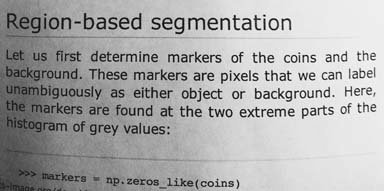
\includegraphics[interpolate=true,width=\textwidth]{images/essentials_binarization_uneven_illumination}
        \caption{Ursprüngliche Grafik~\cite{scikit-image}}%
    \end{subfigure}
    \hfill
    \begin{subfigure}[t]{0.3\textwidth}
        \centering
        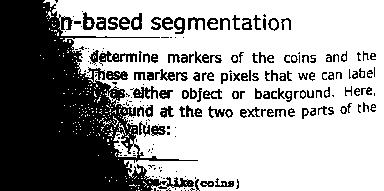
\includegraphics[interpolate=true,width=\textwidth]{images/essentials_binarization_uneven_illumination_otsu}
        \caption{Otsu's Methode\\(Global)}%
    \end{subfigure}
    \hfill
    \begin{subfigure}[t]{0.3\textwidth}
        \centering
        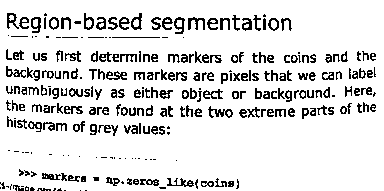
\includegraphics[interpolate=true,width=\textwidth]{images/essentials_binarization_uneven_illumination_sauvola}
        \caption{Sauvola's Methode\\(Lokal)}%
    \end{subfigure}
    \caption{Anpassungsfähigkeit lokaler Schwellenwertfunktionen bei ungleichmäßiger Ausleuchtung}%
    \label{fig:essentials_binarization_uneven_illumination}
\end{figure}

\begin{figure}
    \begin{subfigure}[t]{0.3\textwidth}
        \centering
        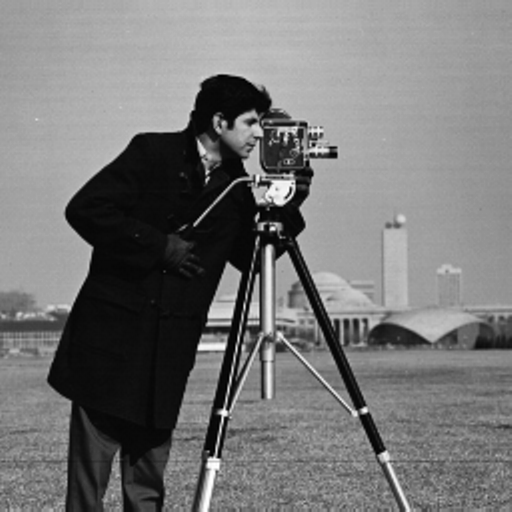
\includegraphics[interpolate=true,width=\textwidth]{images/essentials_binarization_window_size}
        \caption{Ursprüngliche Grafik~\cite{scikit-image}}%
    \end{subfigure}
    \hfill
    \begin{subfigure}[t]{0.3\textwidth}
        \centering
        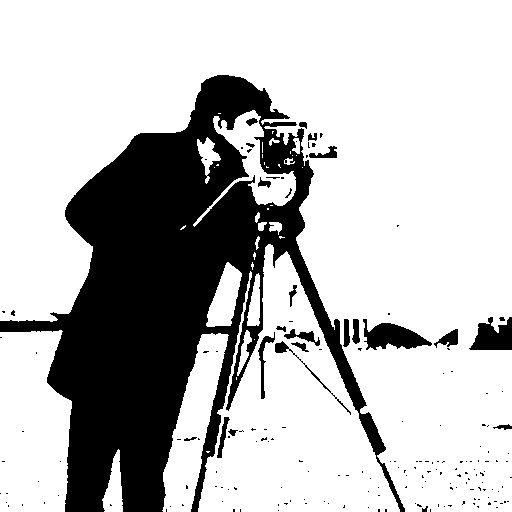
\includegraphics[interpolate=true,width=\textwidth]{images/essentials_binarization_window_size_otsu}
        \caption{Otsu's Methode\\(Global)}%
    \end{subfigure}
    \hfill
    \begin{subfigure}[t]{0.3\textwidth}
        \centering
        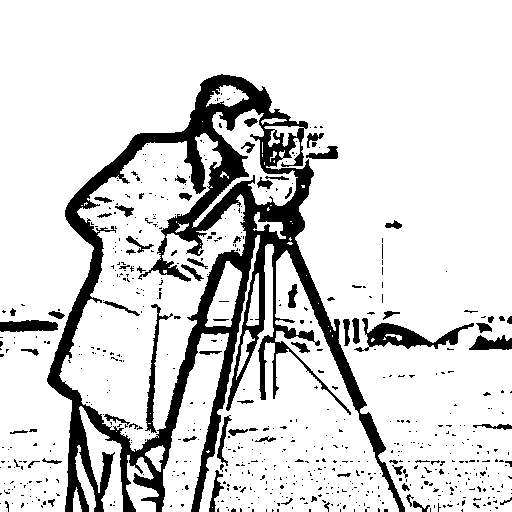
\includegraphics[interpolate=true,width=\textwidth]{images/essentials_binarization_window_size_sauvola}
        \caption{Sauvola's Methode\\(Lokal)}%
    \end{subfigure}
    \caption{Inkorrekte Binarisierung mit lokalen Schwellenwertfunktionen aufgrund zu kleiner Fenstergrößen}%
    \label{fig:essentials_binarization_window_size}
\end{figure}

\clearpage
\subsection{Sauvola's Methode}%
\label{subsec:essentials_binarization_sauvola}

Angenommen folgende Definitionen für Sauvola's Methode~\cite{DBLP:journals/pr/SauvolaP00} gelten:

\begin{tabu}{lX}
    \(w\)      & Fenstergröße des Algorithmus \\
    \(R\)      & Hälfte des Wertebereichs --- Beispielsweise \(128\) für 8-Bit Grafiken \\
    \(k\)      & Faktor des Einflusses der Standardabweichung auf den Schwellenwert \\
    \(m(x,y)\) & Durchschnittlicher Pixelwert im Fenster \((w,w)\) mit \((x,y)\) als Zentrum \\
    \(s(x,y)\) & Standardabweichung der Pixelwerte im Fenster \((w,w)\) mit \((x,y)\) als Zentrum \\
\end{tabu}

Dann wird der Schwellenwert wie folgt berechnet:
\begin{gather}
    T(x,y) = m(x,y) * \left(1 + k * \left(\frac{s(x,y)}{R} - 1\right)\right)
\end{gather}

Unter der Annahme, dass \(k\) ein kleiner, positiver Faktor ist, dann ist bereits ersichtlich wie
\begin{gather*}
    T(x,y) = m(x,y) * \ldots
\end{gather*}
mit dem durchschnittlichen Pixelwert \(m(x,y)\) die Gleichung dominiert und eine Art Basiswert für den Schwellenwert liefert.
\(m(x,y)\) wird im Fenster \((w,w)\) um das Zentrum \((x,y)\) berechnet, weshalb eine Änderung des durchschnittlichen Farbwertes über die Grafik hinweg auch eine Änderung des Schwellenwerts zur Folge hat.
Liegt demzufolge nur ein Teil eines Bildes im Schatten so passt sich Sauvola's Methode den neuen Umständen an.
Hierbei entsteht jedoch das Problem, dass in Bereichen geringer Farbwertvarianz innerhalb der Grafik die Schwelle fälschlicherweise bereits durch geringste Abweichungen unterschritten wird (\autoref{fig:essentials_binarize_without_stddev}).

Deshalb kommt nun die Standardabweichung \(s(x,y)\) zum Einsatz.
Da der Wertebereich der Standardabweichung dem Wertebereich der Grafik entspricht, folgt, dass
\begin{gather*}
    \frac{s(x,y)}{R} = 2
\end{gather*}
und somit der Gleichungsteil
\begin{gather*}
    k * \left(\frac{s(x,y)}{R} - 1\right)
\end{gather*}
einen Wertebereich von \([-k;+k]\) haben muss.

Dies wirkt in der Gleichung als Moderator, der den Schwellenwert, welcher auf dem durchschnittlichen Pixelwert \(m(x,y)\) basiert, um bis zu einem Faktor von \(k\) senken/erhöhen kann, falls die Standardabweichung der Pixel gering/hoch ist.
In Bereichen geringer Farbwertvarianz resultiert es darin, dass die Schwelle abgesenkt und somit nicht unterschritten wird (\autoref{fig:essentials_binarize_with_stddev}).

\begin{figure}[htbp]
    \begin{subfigure}[t]{0.3\textwidth}
        \centering
        
\includegraphics[interpolate=true,width=\textwidth]{images/smiley}
        \caption{Ursprüngliche Grafik}%
        \label{fig:essentials_binarize_input}
    \end{subfigure}
    \hfill
    \begin{subfigure}[t]{0.3\textwidth}
        \centering
        
\includegraphics[interpolate=true,width=\textwidth]{images/essentials_binarization_sauvola_without_stddev}
        \caption{Ohne Einfluss der Standardabweichung}%
        \label{fig:essentials_binarize_without_stddev}
    \end{subfigure}
    \hfill
    \begin{subfigure}[t]{0.3\textwidth}
        \centering
        
\includegraphics[interpolate=true,width=\textwidth]{images/essentials_binarization_sauvola}
        \caption{Mit Einfluss der Standardabweichung}%
        \label{fig:essentials_binarize_with_stddev}
    \end{subfigure}
    \caption{Binarisierung mittels Sauvola's Methode}%
    \label{fig:essentials_binarize}
\end{figure}

\clearpage
\section{Distanztransformation}%
\label{sec:essentials_distance_transform}

\begin{figure}[ht]
    \centering
    \begin{subfigure}[t]{0.45\textwidth}
        \centering
        
\includegraphics[interpolate=false,height=4cm]{images/holsteiner-stute}
    \end{subfigure}
    \hfill
    \begin{subfigure}[t]{0.45\textwidth}
        \centering
        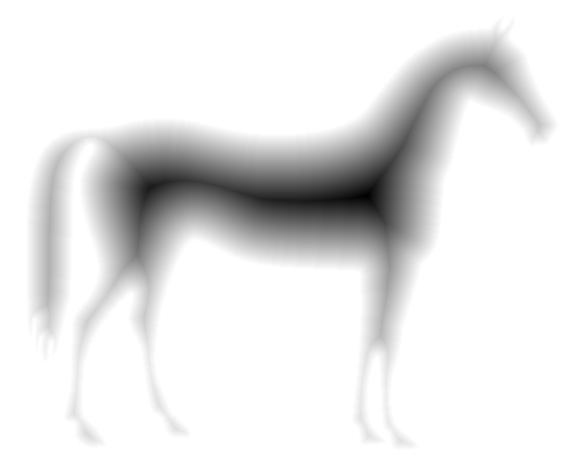
\includegraphics[interpolate=false,height=4cm]{images/essentials_distance_transform_horse}
    \end{subfigure}
    \caption{Eine euklidische Distanztransformation~\cite{DBLP:journals/pami/MaurerQR03,scikit-image}}%
    \label{fig:essentials_distance_transform_horse}
\end{figure}

\wrapfigurefix{0bp}
\begin{wrapfigure}{R}{4cm}
    \hyphenpenalty=0
    \centering
    \includesvg[inkscapelatex=false,inkscapearea=nocrop,width=4cm]{images/essentials_distance_transform}
    \caption{Distanztransformation eines Rechtecks}%
    \label{fig:essentials_distance_transform}
\end{wrapfigure}
Die Distanztransformation berechnet für jeden Vordergrundpixel die kürzeste Distanz zum Bildhintergrund~\cite{DBLP:journals/pr/RosenfeldP68}.
Solch eine Operation bildet die Grundlage für viele weiterführende Algorithmen --- unter anderem auch für die Medial-Achsen Transformation in \autoref{sec:essentials_skeletonization}.
Als Distanzfunktion wird in der Regel die euklidische Distanz benutzt.
Allerdings ist es auch möglich, andere Funktionen zu verwenden --- beispielsweise die Manhatten-Distanz.
\autoref{fig:essentials_distance_transform} zeigt die resultierenden Manhatten-Distanzen beispielhaft anhand eines zum Vordergrund zugehörigen Rechtecks.
\autoref{fig:essentials_distance_transform_horse} zeigt darüber hinaus analog eine euklidische Distanztransformation.
\wrapfigureunfix{}

Eine Brute-Force Berechnung der Distanztransformation ist hierbei ein sehr einfacher Ansatz, bei welchem für jeden Vordergrundpixel separat die geringste Distanz zu allen vorhandenen Hintergrundpixeln berechnet wird.
Solch eine Berechnung hat hierdurch jedoch eine Komplexität von \(\mathcal{O}(n^2)\) (\(n\): Pixelanzahl der Grafik).
Ein entsprechende, exemplarische Implementierung einer euklidischen Distanztransformation ist im Anhang in \autoref{lst:essentials_distance_transform_brute_force} sichtbar.

Im Implementationsteil dieser Arbeit wird später auf eine wesentlich komplexere und fortgeschrittenere Lösung in Form von Felzenszwalb's Methode~\cite{DBLP:journals/toc/FelzenszwalbH12} zurückgegriffen, welche von OpenCV~\cite{opencv_library} implementiert wurde.
Diese berechnet ebenfalls eine exakte euklidische Distanztransformation und liefert somit identische Ergebnisse zur Brute-Force Berechnung.
Anders als der Brute-Force Ansatz kann sie jedoch eine Komplexität von \(\mathcal{O}(n)\) und somit eine signifikant höhere Performanz vorweisen.

\clearpage
\section{Skelettierung}%
\label{sec:essentials_skeletonization}

\begin{figure}[ht]
    \begin{subfigure}[t]{0.48\textwidth}
        \centering
        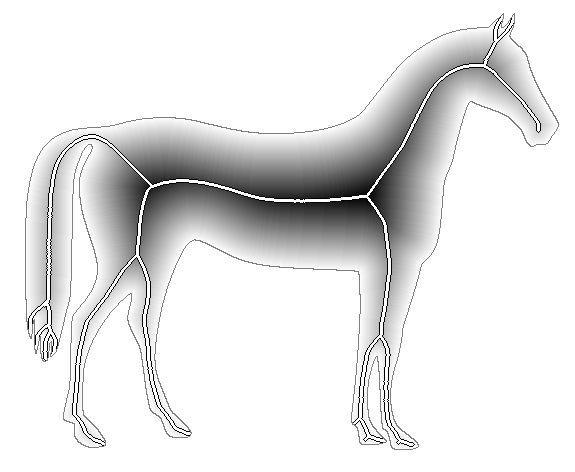
\includegraphics[interpolate=true,width=\textwidth]{images/essentials_skeletonize_medial_axis}
        \caption{Medial-Achsen Transformation, berechnet mit~\cite{scikit-image}}
    \end{subfigure}
    \hfill
    \begin{subfigure}[t]{0.48\textwidth}
        \centering
        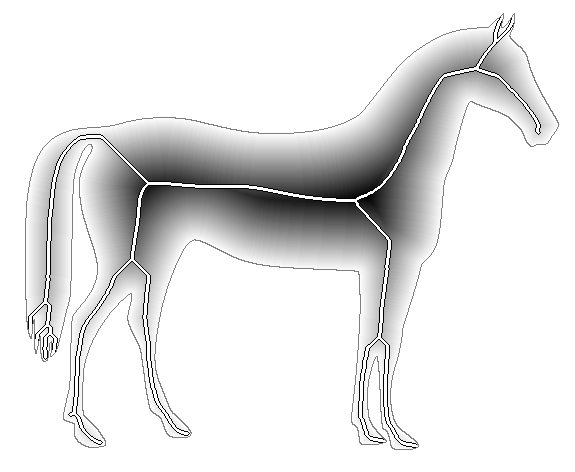
\includegraphics[interpolate=true,width=\textwidth]{images/essentials_skeletonize_thinning}
        \caption{Zhang-Suen Thinning~\cite{DBLP:journals/cacm/ZhangS84}}
    \end{subfigure}
    \caption[Gegenüberstellung zweier prinzipieller Ansätze der Skelettierung]{Gegenüberstellung zweier prinzipieller Ansätze der Skelettierung\\(die Distanztransformation der ursprünglichen Grafik ist im Hintergrund zu sehen)}%
    \label{fig:essentials_skeletonization_comparison}
\end{figure}

Bei der Skelettierung wird eine verdünnte Version einer binären Grafik erzeugt, welche nur noch aus annähernd ein Pixel breiten Linien besteht.
Generell ist es das Ziel, dass jeder Pixel des Skeletts sich möglichst gleich weit entfernt zu den jeweils nächstgelegenen, topologischen Rändern befindet.
Die zügige und gleichzeitig korrekte Ermittlung der Skelettierung in Binärgrafiken ist jedoch schwierig zu erreichen.
Existierende Algorithmen lassen sich deshalb mit zwei potentiellen Eigenschaften einordnen:
\begin{itemize}
    \item Geometrisch korrekt \\
    Das berechnete Skelett befindet sich exakt mittig zwischen den nächstgelegenen topologischen Rändern.
    Diese Eigenschaft bleibt auch dann beibehalten, wenn die Grafik rotiert, skaliert oder anderweitig transformiert wird.
    \item Topologisch korrekt \\
    Das Skelett behält die Topologie der ursprünglichen Grafik bei.
    Die Anzahl der verbundenen Komponenten der Grafik darf entsprechend nicht verändert werden.
\end{itemize}

Die Skelettierung mithilfe von Voronoi-Diagrammen~\cite{DBLP:conf/cvpr/OgniewiczI92} ist als Ausnahme in der Lage, beide Eigenschaften zu besitzen.
Deren Nutzung bleibt jedoch durch den hohen Rechenaufwand in der Regel verwehrt.
In der Praxis werden deshalb üblicherweise andere Herangehensweisen verwendet.

Eine geometrisch korrekte Skelettierung wird in der Regel auf Basis der Gebirgskämme einer Distanztransformation berechnet (siehe \autoref{sec:essentials_distance_transform}).
Solcherlei Herangehensweisen werden als \enquote{Medial-Achsen Transformation}~\cite{Blum:1967:ATF} bezeichnet.
Ein großes Problem ist jedoch die topologische Korrektheit derartiger Algorithmen, da es in der Praxis schwierig ist, alle relevanten Gebirgskämme der Distanztransformation zu extrahieren, ohne gleichzeitig die Skelettierung unnötig zu verkomplizieren.
Neuere Arbeiten fokussieren sich deshalb primär auf eine Verbesserung dieser Situation. (Beispielsweise~\cite{DBLP:journals/cg/MonteroL12}.)

Topologisch korrekte Skelettierungen können jedoch unter anderem mithilfe sogenanntem \enquote{Thinning}~\cite{DBLP:journals/pami/LamLS92} erhalten werden.
Derartige Algorithmen erodieren gezielt die ursprüngliche binäre Grafik sukzessiv, indem jeweils triviale Pixel entfernt werden.
\enquote{Triviale Pixel} sind hierbei jene, welche beim Entfernen nicht die Anzahl der verbundenen Komponenten ändern.
Da die Thinning-Algorithmen einzig die Konnektivität betrachten, kann jedoch zwangsläufig nicht mehr die geometrisch korrekte Platzierung der Skelettierung garantiert werden.

\autoref{fig:essentials_skeletonization_comparison} zeigt Beispielhaft die geometrische Korrektheit einer Medial-Achsen Transformation~\cite{scikit-image} gegenüber dem Zhang-Suen Thinning~\cite{DBLP:journals/cacm/ZhangS84}.

Die vorliegende Arbeit beschäftigt sich mit der Skelettierung von Handzeichnungen bei gleichzeitigem Erhalt der Linienbreite.
Als solches wird es im Entwurfsteil dieser Arbeit (siehe \autoref{cha:theory}) notwendig werden, die Distanztransformation der binarisierten Grafik zu berechnen.
Es ist deshalb naheliegend eine Medial-Achsen Transformation einzusetzen, welche direkt auf der bereits berechneten Distanztransformation aufbaut.
Diese würde darüber hinaus eine geometrisch korrekte Skelettierung und somit eine gute optische Repräsentation der ursprünglichen Grafik garantieren.
Moderne Algorithmen der Medial-Achsen Transformation (beispielsweise~\cite{DBLP:journals/cg/MonteroL12}) konnten in kleineren Testläufen auch stets topologisch korrekte Skelettierungen erzielen.
Jedoch stellte sich die Implementation solcher modernen Algorithmen als zu zeitaufwändig heraus, weshalb die Nutzung der Medial-Achsen Transformation verworfen wurde.
Im folgenden Abschnitt wird deshalb die gewählte, einfachere Alternative in Form des etablierten Zhang-Suen Thinning erläutert.

\subsection{Zhang-Suen Thinning}%
\label{subsec:essentials_skeletonization_zhang_suen}

\wrapfigurefix{0bp}
\begin{wrapfigure}{R}{5cm}
    \centering
    \includesvg[inkscapelatex=false,inkscapearea=nocrop]{images/essentials_zhang_suen_grid}
    \caption{Bezeichnung der Pixelnachbarschaft}%
    \label{fig:essentials_zhang_suen_grid}
\end{wrapfigure}
Einer der bekanntesten Thinning-Algorithmen ist Zhang-Suen's Methode~\cite{DBLP:journals/cacm/ZhangS84}.
Angenommen man betrachtet jedes Pixel \(P_1\) an der Stelle \((x,y)\) der Grafik in einem \((3,3)\) Fenster.
Die Werte der Pixel sind entweder \(0\) für den Bildhintergrund oder \(1\) für den zu erodierenden Bildvordergrund.
Die um \(P_1\) liegenden Pixel werden entsprechend \autoref{fig:essentials_zhang_suen_grid} benannt.
\wrapfigureunfix{}

Zhang-Suen's Methode wird nun sukzessiv triviale Pixel in der Grafik entfernen, beziehungsweise auf \(0\) setzen.
Der Vorgang wird solange wiederholt bis keine Pixel mehr erkannt und entfernt werden können.
Jede Iteration operiert hierbei in zwei sequentiellen Durchläufen.
Tatsächliche Mutationen werden jedoch auf die Grafik erst nach einem Durchlauf angewendet, wodurch es möglich wird den folgenden Algorithmus beliebig zu parallelisieren.

In beiden Durchläufen gilt generell, dass \(P_1\) ein triviales Pixel ist, falls:
\begin{align}
    \label{eq:essentials_zhang_suen_cond_p} & P_1 = 1 \\
    \label{eq:essentials_zhang_suen_cond_a} & A(P_1) = 1 \\
    \label{eq:essentials_zhang_suen_cond_b} & 2 \leq B(P_1) \leq 6
\end{align}
Wobei:
\begin{align}
    A(P_1) &= \text{Anzahl von }0 \to 1\text{ Übergängen in }(P_2, \ldots, P_9) \\
    B(P_1) &= P_2 + \cdots + P_9
\end{align}
Des Weiteren gilt im ersten Durchlauf:
\begin{align}
    \label{eq:essentials_zhang_suen_cond_1}
    \begin{split}
        P_2 * P_4 * P_6 &= 0 \\
        P_4 * P_6 * P_8 &= 0
    \end{split}
\end{align}
Sowie im zweiten Durchlauf:
\begin{align}
    \label{eq:essentials_zhang_suen_cond_2}
    \begin{split}
        P_2 * P_4 * P_8 &= 0 \\
        P_2 * P_6 * P_8 &= 0
    \end{split}
\end{align}

\autoref{eq:essentials_zhang_suen_cond_p} stellt sicher, dass nur Pixel betrachtet werden, welche noch zum Vordergrund gehören.
\autoref{eq:essentials_zhang_suen_cond_a} verhindert, dass \(P_1\) entfernt wird, falls hierdurch die Konnektivität des Skeletts reduziert werden würde (\autoref{fig:essentials_zhang_suen_cond_a}).
\autoref{eq:essentials_zhang_suen_cond_b} verhindert mithilfe von \(2 \leq B(P_1)\)  weiterhin, dass Linienenden unnötig gekürzt werden (\autoref{fig:essentials_zhang_suen_cond_b1}), sowie mit \(B(P_1) \leq 6\), dass fälschlicherweise Löcher in noch nicht vollständig skelettierten Bereichen erzeugt werden (\autoref{fig:essentials_zhang_suen_cond_b7}).

Diese Regelungen ergeben nun insgesamt \(40\) verschiedene Anordnungen in denen Pixel erodiert werden.
Für jede Anordnungen innerhalb der \(40\) lässt sich jeweils eine weitere erlaubte Anordnung finden welche horizontal und/oder vertikal gespiegelt ist (vergleiche \autoref{fig:essentials_zhang_suen_cond_both}, versus \autoref{fig:essentials_zhang_suen_cond_1}).
Jeder Durchlauf betrachtet jedoch jeweils nur \(34\) davon.
Dies ist eine besondere Notwendigkeit für Zhang-Suen Thinning, da aufgrund der \((3,3)\) Fenstergröße eine Situation entstehen kann, in welcher zwei oder mehr spiegelsymmetrische Anordnungen zu zwei oder mehr benachbarten Pixeln passen und somit eine ganze Guppe von Pixeln in einem einzelnen Durchlauf entfernt werden könnte.
Deshalb teilen \autoref{eq:essentials_zhang_suen_cond_1} und \autoref{eq:essentials_zhang_suen_cond_2} jede Iteration in zwei einzelne, eindeutige Durchläufe auf.
Dieser Umstand wird unter anderem in~\cite{DBLP:conf/icpr/ZhangW88a} diskutiert und der Algorithmus zu einem Durchlauf per Iteration verbessert.

\clearpage
\begin{figure}[!htb]
    \centering
    \begin{subfigure}[t]{0.3\textwidth}
        \centering
        \includesvg[inkscapelatex=false,inkscapearea=nocrop,height=1cm]{images/essentials_zhang_suen_both}
        \caption{In beiden Durchläufen zu entfernendes Pixel}%
        \label{fig:essentials_zhang_suen_cond_both}
    \end{subfigure}
    \hfill
    \begin{subfigure}[t]{0.3\textwidth}
        \centering
        \includesvg[inkscapelatex=false,inkscapearea=nocrop,height=1cm]{images/essentials_zhang_suen_first}
        \caption{Im ersten Durchlauf zu entfernendes Pixel}%
        \label{fig:essentials_zhang_suen_cond_1}
    \end{subfigure}
    \hfill
    \begin{subfigure}[t]{0.3\textwidth}
        \centering
        \includesvg[inkscapelatex=false,inkscapearea=nocrop,height=1cm]{images/essentials_zhang_suen_bad_a}
        \caption{Nicht zu entfernendes Pixel, da \(A(P_1) = 2\)}%
        \label{fig:essentials_zhang_suen_cond_a}
    \end{subfigure}

    \begin{subfigure}[t]{0.3\textwidth}
        \centering
        \includesvg[inkscapelatex=false,inkscapearea=nocrop,height=1cm]{images/essentials_zhang_suen_bad_b1}
        \caption{Nicht zu entfernendes Pixel, da \(B(P_1) = 1\)}%
        \label{fig:essentials_zhang_suen_cond_b1}
    \end{subfigure}
    \qquad
    \begin{subfigure}[t]{0.3\textwidth}
        \centering
        \includesvg[inkscapelatex=false,inkscapearea=nocrop,height=1cm]{images/essentials_zhang_suen_bad_b7}
        \caption{Nicht zu entfernendes Pixel, da \(B(P_1) = 7\)}%
        \label{fig:essentials_zhang_suen_cond_b7}
    \end{subfigure}
    \caption{Potentielle Anordnungen beim Zhang-Suen Thinning}
\end{figure}

\subsection{Imperfektionen des Zhang-Suen Thinning}%
\label{subsec:essentials_skeletonization_zhang_suen_imperfection}

\begin{wrapfigure}{R}{5cm}
    \centering
    \includesvg[inkscapelatex=false,inkscapearea=nocrop,height=1cm]{images/essentials_zhang_suen_imperfection}
    \caption{Imperfektion des Zhang-Suen Thinning}%
    \label{fig:essentials_zhang_suen_imperfection}
\end{wrapfigure}
Leider gehört Zhang-Suen Thinning zu jenen Skelettierungsalgorithmen, welche nicht exakt ein Pixel breite Linien erzeugen.
Anordnungen wie in \autoref{fig:essentials_zhang_suen_imperfection} sowie deren \(\lbrace{}90°,180°,270°\rbrace{}\) Rotationen, enthalten den überflüssigen Pixel \textunicode{▨}, welcher ohne Störung der Topologie entfernt werden könnte~\cite{DBLP:journals/pami/LamLS92}.

\clearpage
\section{Douglas-Peucker Kurvenglättung}%
\label{sec:essentials_douglas_peucker}

Der Douglas-Peucker Algorithmus~\cite{doi:10.3138/FM57-6770-U75U-7727} ist ein weit bekannter Ansatz zur Glättung beziehungsweise Approximation von Linienzügen.
Ein Linienzug zwischen zwei Punkten \(P_1\) bis \(P_n\) wird zu der direkten Geraden \(\overline{P_1 P_n}\) vereinfacht, wenn alle Punkte \((P_2, \ldots, P_{n-1})\) einen lotrechten Abstand zur direkten Geraden von höchstens \(d\) haben (siehe \autoref{fig:essentials_douglas_peucker_simple}).
Ist dies nicht der Fall, so wird der Punkt \(P_m\) mit dem größten lotrechten Abstand ermittelt und der Linienzug in die zwei Abschnitte \((P_1, \ldots, P_m)\) und \((P_m, \ldots, P_n)\) aufgeteilt.
Auf beide Abschnitte wird nun derselbe Algorithmus rekursiv angewendet (siehe \autoref{fig:essentials_douglas_peucker_split}).

\mbox{}

\begin{figure}[htbp]
    \centering
    \begin{subfigure}[t]{0.45\textwidth}
        \centering
        \includesvg[inkscapelatex=false,inkscapearea=nocrop,height=6cm]{images/essentials_douglas_peucker_simple}
        \caption{Der gesamte Linienzug befindet sich innerhalb der Grenze \(d\)}%
        \label{fig:essentials_douglas_peucker_simple}
    \end{subfigure}
    \hfill
    \begin{subfigure}[t]{0.45\textwidth}
        \centering
        \includesvg[inkscapelatex=false,inkscapearea=nocrop,height=6cm]{images/essentials_douglas_peucker_split}
        \caption{Ein Punkt \(P_m\) mit dem lotrechten Abstand \(m\) befindet sich außerhalb von \(d\)}%
        \label{fig:essentials_douglas_peucker_split}
    \end{subfigure}
    \caption{Visuelle Darstellung des Douglas-Peucker Algorithmus}
\end{figure}

\clearpage
\section{OpenCV}%
\label{sec:essentials_opencv}

OpenCV~\cite{opencv_library} steht für und ist eine \enquote{Open Source Computer Vision Library}.
Im Bereich der Bildverarbeitung gilt sie als eine allgemein bekannte und angesehene Bibliothek und bietet optimierte Implementationen einer Vielzahl an grundlegenden Imperativen sowie moderner Algorithmen.

Beispielsweise liest der folgende \texttt{C++} Code eine Bilddatei namens \texttt{input.jpg} ein, wendet den Gaußschen Weichzeichner mit einer Fenstergröße von \((3,3)\) an und speichert das Ergebnis als \texttt{output.jpg} ab:
\begin{minted}[gobble=4]{cpp}
    cv::Mat input = cv::imread("input.jpg");
    cv::Mat output;
    cv::blur(input, output, {3, 3});
    cv::imwrite("output.jpg", output);
\end{minted}

\texttt{cv::Mat} ist eine OpenCV Klasse, welche n-Dimensionale Matrizen verwaltet und steht in der Bibliothek an zentraler Stelle.
Liest man eine Bilddatei ein wird auch diese in einer solchen Matrix gespeichert (siehe Zeile 1).
So wie die meisten Funktionen in OpenCV ist dadurch auch die auf Zeile 3 verwendete \texttt{cv::blur} Funktion nur noch die abstrakte Transformation einer Matrix.

Zusätzlich bieten neuere Versionen von OpenCV die leicht abgewandelte Klasse \texttt{cv::UMat}.
Wird diese an Stelle von \texttt{cv::Mat} verwendet, können viele grundlegende Funktionen --- unter anderem auch \texttt{cv::blur} --- eine potentiell existierende GPU des Computers für eine starke Beschleunigung nutzen.

Da OpenCV nicht nur bereits zwei verschiedene Container-Klassen für Matrizen, sondern auch einige andere Formate unterstützen muss, sind die meisten Funktionen in OpenCV in etwa wie folgt definiert:
\begin{minted}[gobble=4]{cpp}
    void transformation(cv::InputArray source, cv::OutputArray destination);
\end{minted}

\texttt{cv::InputArray} speichert eine konstante Referenz zu einem der unterstützten Container-Klassen ab.
Es ist nachträglich möglich abzufragen, welche Art von Container das \texttt{cv::InputArray} speichert, weshalb die jeweilige Funktion sich zum Beispiel auf eine GPU-Beschleunigung spezialisieren kann, sofern der Aufrufer zur Laufzeit eine \texttt{cv::UMat} Instanz übergeben hat.
\texttt{cv::InputArray} stellt somit eine Art von manueller, dynamischer Polymorphie dar.

\texttt{cv::OutputArray} ist das entsprechende Gegenstück mit identischen Fähigkeiten.
Jedoch wird hierbei eine mutable Referenz gespeichert, in welcher das Ergebnis der Transformation gespeichert werden kann.

\chapter{Entwurf}%
\label{cha:theory}

Ziel der vorliegenden Arbeit ist es, eine Programmbibliothek zu entwickeln, welche fotografierte Handzeichnungen vektorisiert.
Um mit der internen Repräsentation der Mobilanwendung Mind-Objects kompatibel zu sein, ist es notwendig, dass die aus der Vektorisierung resultierenden Linien nur mithilfe ihrer polygonalen Mittellinie sowie der variierenden Linienbreite, beziehungsweise Radien, repräsentiert werden (siehe \autoref{fig:theory_line_radius}).
Bei der späteren Darstellung verknüpft die Anwendung die Punkte mit einzelnen Linien, deren Breite den Radien der Punkte entsprechen.
Als Endergebnis des Gesamtprozess sollte die optische Darstellung der rekonstruierten Linien annähernd der ursprünglichen fotografierten Handzeichnung entsprechen.

\begin{figure}[h]
    \centering
    \begin{subfigure}[t]{0.45\textwidth}
        \includesvg[inkscapelatex=false,inkscapearea=nocrop,width=\textwidth]{images/theory_line_radius}
        \caption{\textcolor{gray}{\textunicode{●}}~Ursprüngliche Linie\enskip\textunicode{●}~Mittellinie\enskip\textunicode{◍}~Linienbreite}
    \end{subfigure}
    \hfill
    \begin{subfigure}[t]{0.45\textwidth}
        \includesvg[inkscapelatex=false,inkscapearea=nocrop,width=\textwidth]{images/theory_line_radius_reconstructed}
        \caption{\textcolor{gray}{\textunicode{●}}~Rekonstruierte Linie\enskip\textunicode{●}~Knotenpunkte\enskip\textunicode{◍}~Radien}
    \end{subfigure}
    \caption{Zielstellung der Linienrepräsentation}%
    \label{fig:theory_line_radius}
\end{figure}

Im Bereich der Grafik-Vektorisierung existieren eine Vielzahl von Ansätzen, die für diese Arbeit in Frage kommen könnten.
Als gebräuchlichster Ablauf gilt jedoch~\cite{DBLP:journals/pami/HilaireT06,DBLP:conf/grec/TombreADMT99}:
\begin{itemize}
    \item Linien in der Rastergrafik finden
    \item Diese Linien in einzelne vektorisierte Primitiven segmentieren
    \item Kontextuelles Wissen der Fotografie nutzen um das Ergebnis aufzubessern
\end{itemize}

\clearpage
Für das Auffinden von Linien in der Rastergrafik stehen prinzipiell drei Arten von Algorithmen zur Verfügung:
\begin{itemize}
    \item Anpassung parametrischer Figuren \\
    Mithilfe eines passenden Modells können Algorithmen wie die Hough Transformation~\cite{DBLP:journals/cacm/DudaH72} Linien im Bild erkennen.
    Es existieren jedoch nur wenige Ansätze zur Vektorisierung dieser Art (beispielsweise~\cite{DBLP:journals/pr/SongL05}).
    Der größte Nachteil ist die inhärente Eigenschaft solcher Algorithmen, ausschließlich jene Figuren zu erkennen, welche das Modell vorgibt.
    Eine flexible Lösung zur Erkennung von beliebigen Linienzügen ist deshalb schwieriger zu erreichen.
    \item Parallele Gegenkonturen erkennen \\
    Nach der Anwendung eines Algorithmus zur Kantendetektion --- beispielsweise Canny's Methode~\cite{DBLP:journals/pami/Canny86a} --- können gegenüberliegende, annähernd parallele Konturen zu Linien zusammengefasst werden.
    Die Distanz zwischen den beiden Konturen entspricht dann der Linienbreite.
    Algorithmen wie die Stroke-Width Transformation~\cite{DBLP:conf/cvpr/EpshteinOW10} nutzen solch einen Ansatz im Bereich der Texterkennung, da Algorithmen zur Kantendetektion äußerst zuverlässig auch schwach ausgeprägte Konturen von Schriftzügen erkennen.
    Schriftzüge setzen sich aus Linien annähernd konstant bleibender Breite zusammen.
    Indem diejenigen ermittelten parallelen Konturen entfernt werden, welche keine konstante Linienbreite vorweisen, kann daher das Ergebnis im Kontext der Texterkennung aufgebessert werden.
    Problematisch ist allerdings, dass sich bei Linienkreuzungen unter Umständen keine parallelen Konturen finden lassen.
    Ist also nicht eine Texterkennung das Ziel, sondern eine generelle Vektorisierung von Handzeichnungen, so verkompliziert sich die Lösungsfindung für uneindeutige Konturen, wodurch komplexe Heuristiken und Algorithmen notwendig werden.
    \item Skelettierungen \\
    Skelettierungsalgorithmen reduzieren eine binäre Grafik auf annähernd ein Pixel breite Mittellinien (siehe \autoref{sec:essentials_skeletonization}).
    Algorithmen wie zum Beispiel die Medial-Achsen Transformation liefern hierbei nicht nur die Mittellinie, sondern sogar auch gleichzeitig die benötigte Linienbreite.
    Aufgrund dessen, sowie der in der Regel relativ simplen Algorithmen, sind Skelettierungen die momentan gebräuchlichste Vorstufe für eine Vektorisierung.
    Nachteilhaft ist jedoch der Umstand, dass hierfür eine Binarisierung (siehe \autoref{sec:essentials_binarization}) notwendig wird.
    Diese sind nicht nur in der Regel äußerst rechenaufwändig, sondern können auch, gegenüber Algorithmen zur Kantendetektion, schwach ausgeprägte Konturen übersehen.
    Skelettierungsalgorithmen können darüber hinaus überflüssige Linienzüge für komplexe Figuren produzieren, ohne deren Existenz eine darauf aufbauende Vektorisierung dennoch korrekt wäre.
    Da für die vorliegende Arbeit aber einzig die optisch korrekte Darstellung im Endergebnis ist, stellen überflüssige Linienzüge kein Problem dar.
\end{itemize}

Während der Ansatz zur Erkennung paralleler Gegenkonturen vielversprechend ist, stellt die hohe Komplexität zur Auflösung von uneindeutigen Konturen im Rahmen dieser Arbeit ein Problem dar.
Skelettierungsalgorithmen bieten hingegen eine weit etablierte, einfache und robuste Alternative, weshalb sie im Folgenden als Ansatz ausgewählt wurden (siehe \autoref{sec:essentials_skeletonization}).
Es existieren hierfür Algorithmen, die eine sogenannte geometrisch korrekte Skelettierung produzieren, deren rekonstruierte, optische Darstellung dem Original sehr nahekommen würde.
Diese basieren üblicherweise auf dem Konzept der Medial-Achsen Transformation, welche sowohl die Skelettierung als auch die notwendige Linienbreite liefern könnte.
\autoref{sec:theory_preprocess} dieses Kapitels wird im Detail auf die Berechnung der Mittellinien und Radien eingehen.

Die mithilfe der Skelettierung berechneten Linien sind noch als Rastergrafik vorhanden.
Es folgt deshalb die Segmentierung der Linien um vektorisierte Primitiven zu erhalten.
Da einzig polygonale Mittellinien berechnet werden sollen, kann dafür ein sehr einfacher Algorithmus entworfen werden.
Dieser muss nur die Segmente der Skelettierung, die keine Linienkreuzungen haben, zu eindeutigen, polygonalen Linienzügen \enquote{aufreihen}.
In \autoref{sec:theory_segmentation} wird dieses Teilproblem näher behandelt.

Letztendlich ist es üblich, die Vektorisierung mithilfe des kontextuellen Wissens des Subjekts, beziehungsweise der Fotografie, aufzubessern.
Während beispielsweise im Bereich der Texterkennung von gewissen Prämissen ausgegangen werden kann --- unter anderem, dass Buchstaben mit annähernd konstanter Strichstärke geschrieben werden, oder dass sie annähernd Quadratisch sind --- stellt sich dies im Falle der Vektorisierung beliebiger Freihandzeichnungen als schwieriges Problem dar.
Deshalb wurde im Rahmen der vorliegenden Arbeit auf die Erstellung eines Algorithmus zur Verbesserung der Vektorisierung zunächst verzichtet.
Trotz dessen ist aber ein Nachbereitungsschritt notwendig: Da im vorherigen Schritt polygonale Linienzüge basierend auf der Skelettierung generiert wurden, enthalten sie einen Knotenpunkt per Pixel der Skelettierung.
Solch eine hohe Menge von Knotenpunkten kann potentiell die Darstellungsgeschwindigkeit der Mobilanwendung negativ beeinflussen.
In \autoref{sec:theory_postprocess} wird deshalb ein Glättungsalgorithmus entworfen, welcher die Linienzüge mit einer Approximation vereinfacht, die optisch ähnlich sind, aber signifikant weniger Knotenpunkte enthalten.

Der aus den nachfolgenden Abschnitten resultierende Ablauf ist in \autoref{sec:theory_flow} zu sehen.

\clearpage
\section{Aufbereitung der Rastergrafik}%
\label{sec:theory_preprocess}

Im vorherigen Abschnitt wurde der generelle Ablauf der Vektorisierung festgelegt.
Als erster Schritt soll die Ermittlung von Linien in der Rastergrafik erfolgen.
Für diesen Zweck wurde der Weg über eine Skelettierung als Lösungsansatz ausgewählt.
Letztendliches Ziel der Arbeit ist es, die vektorisierten Linien mithilfe von polygonalen Mittellinien und deren Radien zu repräsentieren.
Die Gruppe der Algorithmen, welche auf der Medial-Achsen Transformation basieren, bieten exakt solch eine Fähigkeit und liefern gleichzeitig beide benötigten Parameter.
Während der Implementation dieser Arbeit stellten sich derartige, akzeptable Algorithmen (beispielsweise~\cite{DBLP:journals/cg/MonteroL12}) allerdings als zu aufwändig heraus.
Obwohl die Distanztransformation weiterhin benötigt wird und deshalb auch weiterhin berechnet werden muss, wurde sich temporär für einen einfacheren Ansatz in Form vom Zhang-Suen Thinning~\cite{DBLP:journals/cacm/ZhangS84} entschieden (siehe \autoref{subsec:essentials_skeletonization_zhang_suen}).
Zhang-Suen's Methode ist einer der bekanntesten Thinning-Algorithmen, lässt sich sehr leicht implementieren und bietet für einen ersten Ansatz der Vektorisierung Ergebnisse, die einer korrekteren Medial-Achsen Transformation nahe genug kommen~\cite{DBLP:journals/pami/LamLS92}.

Eine derartige Rekonstruktion einer Grafik aus der Skelettierung und der Distanztransformation ist in \autoref{fig:theory_preprocess_reconstructed} sichtbar.
Dabei wurde für jeden schwarzen Pixel der Skelettierung (\autoref{fig:theory_preprocess_skeleton}) ein Kreis mit dem Radius, entsprechend dem Wert der Distanztransformation (\autoref{fig:theory_preprocess_distance}), gezeichnet.

Wie die meisten Skelettierungsalgorithmen, operiert Zhang-Suen Thinning hingegen auf Binärgrafiken.
Es ist daher zunächst notwendig, die gegebene Fotografie zu binarisieren.
\autoref{sec:essentials_binarization} erläutert die generellen Kategorien von Binarisierungsalgorithmen.
Während Algorithmen mit einer globalen Schwellenfunktion nicht nur sehr performant sind, sondern es auch ermöglichen würden, Linien beliebiger Breite zu vektorisieren, erzielen sie häufig relativ schlechte Ergebnisse bei Fotografien unter natürlichen Lichtverhältnissen, beziehungsweise generell bei Aufnahmen mit inkonsistenter Beleuchtungsstärke.
Deshalb wird ein langsamerer aber robusterer Algorithmus mit lokaler Schwellenfunktion eingesetzt.
Als Algorithmus kommt hierbei Sauvola's Methode zum Einsatz, da diese nicht nur simpel zu implementieren ist, sondern auch gute Ergebnisse bei der Binarisierung von Textdokumenten erzielt~\cite{DBLP:journals/jei/SezginS04}.

Als Ergebnis der Aufbereitung der Grafik liegen die ermittelten Linien, in Form der Skelettierung sowie der Distanztransformation vor.
Es folgt nun die Segmentierung, welche die Skelettierung in einzelne polygonale Linienabschnitte zerlegt, wodurch vektorisierte Linienzüge ermittelt werden.

\begin{figure}[h]
    \begin{subfigure}[t]{0.45\textwidth}
        \centering
        
\includegraphics[height=4cm,interpolate=false]{images/theory_preprocess_skeleton}
        \caption{Skelettierung durch Zhang-Suen Thinning}%
        \label{fig:theory_preprocess_skeleton}
    \end{subfigure}
    \hfill
    \begin{subfigure}[t]{0.45\textwidth}
        \centering
        
\includegraphics[height=4cm]{images/theory_preprocess_distance}
        \caption{Euklidische Distanztransformation}%
        \label{fig:theory_preprocess_distance}
    \end{subfigure}

    \begin{subfigure}[t]{0.45\textwidth}
        \centering
        
\includegraphics[height=4cm]{images/essentials_binarization_sauvola}
        \caption{Binarisiertes Originalbild}
    \end{subfigure}
    \hfill
    \begin{subfigure}[t]{0.45\textwidth}
        \centering
        
\includegraphics[height=4cm]{images/theory_preprocess_reconstructed}
        \caption{Rekonstruktion}%
        \label{fig:theory_preprocess_reconstructed}
    \end{subfigure}
    \caption{Beispiel der Rekonstruktion einer Grafik aus Skelettierung und Distanztransformation}
\end{figure}

\clearpage
\section{Segmentierung}%
\label{sec:theory_segmentation}

Der zu erstellende Prozess soll vektorisierte, polygonale Linien erzeugen, weshalb ein Algorithmus notwendig ist, welcher die Pixel der Skelettierung des vorherigen Abschnitts in geordnete Linienzüge segmentiert.
Da die Skelettierung eine annähernd ein Pixel breite Linie ist, liegt der Ansatz nahe, beginnend von einem beliebigen Vordergrundpixel (hier: schwarzen Pixel) der Skelettierung und mithilfe einer Tiefensuche, sukzessiv \enquote{Pfade} von angrenzenden Pixeln zu bilden.
Dies kann wiederholt werden, bis alle Pixel der Skelettierung Pfaden zugewiesen wurden.
Die Linienbreite der Segmente, beziehungsweise \enquote{Pfade}, entspricht wie bei der Medial-Achsen Transformation dem Wert der Distanztransformation an der jeweiligen Stelle des Skelettierungspixels.

\autoref{fig:theory_segmentation_simple} zeigt einen sehr einfachen Fall, bei welchem die maximale Konnektivität von jedem Pixel maximal \(2\) beträgt und somit für jeden Pixel entlang des Pfades maximal ein Folgepixel gefunden werden kann.

Es stellt sich allerdings die Frage, was im Falle einer Gabelung entlang des Pfades und somit einer Konnektivität von über \(2\) zu tun ist.
Für beispielsweise \autoref{fig:theory_segmentation_intersection} muss deshalb eine Lösung gefunden werden, um \textunicode{◆} als Gabelung zu erkennen und den Pfad nach \textunicode{■}~und~\textunicode{□} aufzuzweigen.

Es ergibt sich darüber hinaus das Problem, dass einige Thinning-Algorithmen nur annähernd ein Pixel breite Linien erzeugen.
Hierzu gehört unter anderem auch das verwendete Zhang-Suen Thinning, welches \enquote{Stufen} bei Diagonalen hinterlässt (siehe \autoref{subsec:essentials_skeletonization_zhang_suen_imperfection}).
Für Fälle wie in \autoref{fig:theory_segmentation_zhang_suen_steps} ist es deshalb notwendig, derartige \enquote{Stufen} zu erkennen und sie korrekt zu ein und derselben Linie zuzuordnen.

Hierbei muss außerdem darauf geachtet werden, dass in Fällen wie in \autoref{fig:theory_segmentation_direction} zu Beginn keine \enquote{Abkürzung} über die zwei Pixel \textunicode{▨} genommen wird.
Diese liegen zwar aneinander, jedoch ist dieser Umstand dem Zhang-Suen Thinning geschuldet, da der Startpunkt gar nicht existieren sollte.

Letztendlich ist es auch notwendig Zyklen wie in \autoref{fig:theory_segmentation_cycle} zu erkennen, da das Ende des Pfads ohne optische Fehler überlappend an den Anfang anknüpfen muss.
Eine Lösung hierfür ist recht simpel: Wird ein vorheriger Startpunkt oder eine Weggabelung erkannt, so wird diese noch als letzter Schritt zum aktuellen Pfad hinzugefügt.

\clearpage
\begin{figure}[!htbp]
    \begin{subfigure}[t]{0.45\textwidth}
        \centering
        \includesvg[inkscapelatex=false,inkscapearea=nocrop,height=25mm]{images/theory_segmentation_simple_path}
    \end{subfigure}
    \hfill
    \begin{subfigure}[t]{0.45\textwidth}
        \centering
        \includesvg[inkscapelatex=false,inkscapearea=nocrop,height=25mm]{images/theory_segmentation_simple_path_traced}
    \end{subfigure}
    \caption[Simple Pfadfindung]{Simple Pfadfindung\protect\footnotemark}%
    \label{fig:theory_segmentation_simple}
\end{figure}
\begin{figure}[!htbp]
    \begin{subfigure}[t]{0.45\textwidth}
        \centering
        \includesvg[inkscapelatex=false,inkscapearea=nocrop,height=25mm]{images/theory_segmentation_intersection}
    \end{subfigure}
    \hfill
    \begin{subfigure}[t]{0.45\textwidth}
        \centering
        \includesvg[inkscapelatex=false,inkscapearea=nocrop,height=25mm]{images/theory_segmentation_intersection_traced}
    \end{subfigure}
    \caption[Pfadfindung trotz Weggabelungen]{Pfadfindung trotz Weggabelungen\protect\footnotemark[\value{footnote}]}%
    \label{fig:theory_segmentation_intersection}
\end{figure}
\begin{figure}[!htbp]
    \begin{subfigure}[t]{0.45\textwidth}
        \centering
        \includesvg[inkscapelatex=false,inkscapearea=nocrop,height=20mm]{images/theory_segmentation_zhang_suen_steps}
    \end{subfigure}
    \hfill
    \begin{subfigure}[t]{0.45\textwidth}
        \centering
        \includesvg[inkscapelatex=false,inkscapearea=nocrop,height=20mm]{images/theory_segmentation_zhang_suen_steps_traced}
    \end{subfigure}
    \caption[Pfadfindung trotz Imperfektionen]{Pfadfindung trotz Imperfektionen\protect\footnotemark[\value{footnote}]}%
    \label{fig:theory_segmentation_zhang_suen_steps}
\end{figure}
\begin{figure}[!htbp]
    \begin{subfigure}[t]{0.45\textwidth}
        \centering
        \includesvg[inkscapelatex=false,inkscapearea=nocrop,height=25mm]{images/theory_segmentation_direction}
    \end{subfigure}
    \hfill
    \begin{subfigure}[t]{0.45\textwidth}
        \centering
        \includesvg[inkscapelatex=false,inkscapearea=nocrop,height=25mm]{images/theory_segmentation_direction_traced}
    \end{subfigure}
    \caption[Pfadfindung trotz anderer Startpunktnachbarn]{Pfadfindung trotz anderer Startpunktnachbarn\protect\footnotemark[\value{footnote}]}%
    \label{fig:theory_segmentation_direction}
\end{figure}
\begin{figure}[!htbp]
    \begin{subfigure}[t]{0.45\textwidth}
        \centering
        \includesvg[inkscapelatex=false,inkscapearea=nocrop,height=20mm]{images/theory_segmentation_cycle}
    \end{subfigure}
    \hfill
    \begin{subfigure}[t]{0.45\textwidth}
        \centering
        \includesvg[inkscapelatex=false,inkscapearea=nocrop,height=20mm]{images/theory_segmentation_cycle_traced}
    \end{subfigure}
    \caption[Pfadfindung trotz Zyklen]{Pfadfindung trotz Zyklen\protect\footnotemark[\value{footnote}]}%
    \label{fig:theory_segmentation_cycle}
\end{figure}
\footnotetext{
    \textunicode{●}~Start\enskip%
    \textunicode{■}/\textunicode{□}~Ende\enskip%
    \textunicode{◆}~Gabelung\enskip%
    \textunicode{▨}~Ignorierte Nachfolger%
    \label{fn:theory_segmentation_symbols}%
}

\clearpage
Es seien folgende Symbole und Farben definiert:

\begin{tabu}{lX}
    \textunicode{●} & Aktuell zu betrachtendes Pixel \\
    \textunicode{■} & Bereits zu einem Pfad zugehöriges Pixel \\
    \textcolor{gray}{\textunicode{■}}/\textcolor{gray}{\textunicode{▨}} & Potentielle Nachfolger \\
\end{tabu}

\begin{figure}[ht]
    \begin{subfigure}[t]{0.3\textwidth}
        \centering
        \includesvg[inkscapelatex=false,inkscapearea=nocrop,height=15mm]{images/theory_segmentation_mask_none}
        \caption{Ohne Nachfolger}%
        \label{fig:theory_segmentation_mask_none}
    \end{subfigure}
    \hfill
    \begin{subfigure}[t]{0.3\textwidth}
        \centering
        \includesvg[inkscapelatex=false,inkscapearea=nocrop,height=15mm]{images/theory_segmentation_mask_one}
        \caption{Eindeutiger Nachfolger}%
        \label{fig:theory_segmentation_mask_one}
    \end{subfigure}
    \hfill
    \begin{subfigure}[t]{0.3\textwidth}
        \centering
        \includesvg[inkscapelatex=false,inkscapearea=nocrop,height=15mm]{images/theory_segmentation_mask_non_adjacent}
        \caption{Uneindeutige\\Nachfolger}%
        \label{fig:theory_segmentation_mask_non_adjacent}
    \end{subfigure}

    \begin{subfigure}[t]{0.3\textwidth}
        \centering
        \includesvg[inkscapelatex=false,inkscapearea=nocrop,height=15mm]{images/theory_segmentation_mask_two}
        \caption{Zhang-Suen Thinning Imperfektion A}%
        \label{fig:theory_segmentation_mask_two}
    \end{subfigure}
    \hfill
    \begin{subfigure}[t]{0.3\textwidth}
        \centering
        \includesvg[inkscapelatex=false,inkscapearea=nocrop,height=15mm]{images/theory_segmentation_mask_three}
        \caption{Zhang-Suen Thinning Imperfektion B}%
        \label{fig:theory_segmentation_mask_three}
    \end{subfigure}
    \hfill
    \begin{subfigure}[t]{0.3\textwidth}
        \centering
        \includesvg[inkscapelatex=false,inkscapearea=nocrop,height=15mm]{images/theory_segmentation_mask_direction}
        \caption{Direktionale Suche}%
        \label{fig:theory_segmentation_mask_direction}
    \end{subfigure}
    \caption{Potentielle Anordnungen der Suchmaske}
\end{figure}

Alle verbleibenden Problemstellungen lassen sich lösen, wenn man jeden Pixel, analog zum Zhang-Suen Thinning (siehe \autoref{sec:essentials_skeletonization}), in einem \((3,3)\) Fenster betrachtet.

Zunächst muss hierbei \autoref{fig:theory_segmentation_simple} algorithmisch gelöst werden.
Wie bereits eingangs erwähnt, werden wir hierfür eine Tiefensuche nutzen um jeweils angrenzende Pixelnachbarn zu einem möglichst langen Pfad zu sammeln.
Die Tiefensuche ist an einem Ende angekommen, wenn man bereits zu einem Pfad zugehörige Pixel (\textunicode{■}) ignoriert und sich wie in \subref{fig:theory_segmentation_mask_none} kein potentieller Nachfolger mehr finden lässt.
Alternativ ergibt sich im einfachsten Fall ein Bild wie in \subref{fig:theory_segmentation_mask_one}, da hier nur ein einziger potentieller Nachfolger (\textcolor{gray}{\textunicode{■}}) verbleibt, welcher dann als Fortsetzung der Tiefensuche dient.

Weggabelungen wie in \autoref{fig:theory_segmentation_intersection} können dadurch erkannt werden, dass zwei oder mehr getrennt voneinander liegende potentielle Nachfolger (\textcolor{gray}{\textunicode{■}}) vorzufinden sind \subref{fig:theory_segmentation_mask_non_adjacent}.
Ist dies der Fall, muss die Tiefensuche beendet werden, da hiermit auch der bisher eindeutige Pfad an dieser Stelle endet.
Allerdings müssen nun, ausgehend von dieser Stelle, für jeden Nachfolger separat Tiefensuchen gestartet werden, damit jene für sich jeweils Pfade generieren.
Auf diese Weise werden ausschließlich eindeutige Pfadsegmente erzeugt.

Imperfektionen der Zhang-Suen Skelettierung, wie in \autoref{fig:theory_segmentation_zhang_suen_steps}, äußern sich durch Anordnungen von mindestens zwei konsekutiv aufeinanderfolgenden Nachbarn (\textcolor{gray}{\textunicode{■}}/\textcolor{gray}{\textunicode{▨}}), von denen jeweils der horizontale oder vertikale Nachbar überflüssig ist (\textcolor{gray}{\textunicode{▨}})~\cite{DBLP:journals/pami/LamLS92}.
\subref{fig:theory_segmentation_mask_two} und \subref{fig:theory_segmentation_mask_three} stellen dies beispielhaft dar --- die horizontalen und vertikalen Spiegelungen sowie jeweiligen \(90°\) Rotationen sind weitere potentielle Kombinationen.

Werden konsekutiv aufeinanderfolgende Nachbarn erkannt, so müssen horizontale und vertikale Nachbarn (\textcolor{gray}{\textunicode{▨}}) favorisiert und als potentieller Nachfolger genutzt werden.
Wenn anschließend solch ein Nachfolger (\textcolor{gray}{\textunicode{▨}}) in der nächsten Iteration behandelt wird, können aufgrund der verbleibenden Prämissen des Zhang-Suen Thinnings, im Fall von \subref{fig:theory_segmentation_mask_two} nur \subref{fig:theory_segmentation_mask_one}, \subref{fig:theory_segmentation_mask_non_adjacent} und \subref{fig:theory_segmentation_mask_three} folgen.
Im Fall von \subref{fig:theory_segmentation_mask_three} hingegen wird der Nachfolger (\textcolor{gray}{\textunicode{▨}}) immer mit der Suchmaske \subref{fig:theory_segmentation_mask_non_adjacent} enden, da die beiden regulären Nachbarn (\textcolor{gray}{\textunicode{■}}) daraufhin getrennt voneinander liegen.
In maximal 2 Folgeiterationen wird dieses Problem somit umgangen und korrekt zu einem Pfad umgewandelt.

Letztendlich kann \autoref{fig:theory_segmentation_direction} gelöst werden, indem zusätzlich die aktuelle \enquote{Richtung} der Suche einbezogen wird.
Hiermit müssen nur die 5 tatsächlich relevanten statt aller 8 Nachbarn im \((3,3)\) Fenster betrachtet werden.
\subref{fig:theory_segmentation_mask_direction} zeigt dies an einem Beispiel:
Beginnend vom Startpunkt \textunicode{■} wurde hier zunächst der rechte Pixel \textunicode{●} ausgewählt.
Dieser ist nun der aktuell zu betrachtende Pixel.
Entsprechend der \enquote{Richtung} des vorherigen Schritts, können weitere Nachfolger nur im, mit der gestrichelten Linie  \textunicode{┅}, umrahmten Bereich vorhanden sein, wodurch nur \textcolor{gray}{\textunicode{■}} in Frage kommt.
Der andere Nachbar des Startpunkts \textcolor{gray}{\textunicode{▨}} wird nicht weiter betrachtet und somit der aktuelle Punkt nicht fälschlicherweise als Weggabelung, wie in \subref{fig:theory_segmentation_mask_non_adjacent}, gekennzeichnet.

Die in diesem Abschnitt erläuterte Segmentierung zerlegt die Skelettierung des vorherigen \autoref{sec:theory_preprocess} in einzelne, vektorisierte, polygonale Linienabschnitte.
Diese sind noch in einer unnötig hohen Auflösung, da der in diesem Abschnitt entwickelte Algorithmus für jeden Pixel einen Knotenpunkt erzeugt hat.
Im Folgenden wird deshalb ein Algorithmus kreiert, welcher die Linienzüge approximiert und optisch unnötige Knotenpunkte entfernt.

\clearpage
\section{Nachbereitung der Vektorisierung}%
\label{sec:theory_postprocess}

Die im vorherigen \autoref{sec:theory_segmentation} ermittelten Liniensegmente enthalten für jeden Pixel der Skelettierung einen Knotenpunkt, beziehungsweise Vertex, welcher dann von der Anwendung gezeichnet wird.
Da die beobachtbare Geschwindigkeit von Grafikanwendungen in der Regel proportional zur Anzahl der sichtbaren und somit zu zeichnenden Knotenpunkten ist, liegt es nahe, jene unbedeutenden Linienpunkte zu entfernen, welche nicht zum Gesamteindruck des Bildes beitragen.
\autoref{fig:theory_postprocess_simplification} zeigt exemplarisch die Reduktion der Anzahl der Knotenpunkte eines im vorherigen Abschnitt ermittelten Linienzugs auf ein Elftel.
Trotz der Approximation sind beide Linienzüge annähernd gleich, ungeachtet dessen, dass der Bildausschnitt stark vergrößert wurde.

\begin{figure}[ht]
    \begin{subfigure}[t]{0.45\textwidth}
        \centering
        \includesvg[inkscapelatex=false,inkscapearea=nocrop,width=\textwidth]{images/theory_postprocess_without_simplification}
        \caption{\(124\) Linienpunkte}
    \end{subfigure}
    \hfill
    \begin{subfigure}[t]{0.45\textwidth}
        \centering
        \includesvg[inkscapelatex=false,inkscapearea=nocrop,width=\textwidth]{images/theory_postprocess_with_simplification}
        \caption{\(11\) Linienpunkte}
    \end{subfigure}
    \caption{Entfernung optisch irrelevanter Linienpunkte}%
    \label{fig:theory_postprocess_simplification}
\end{figure}

\wrapfigurefix{2bp}
\begin{wrapfigure}{R}{5cm}
    \centering
    \includesvg[inkscapelatex=false,inkscapearea=nocrop,width=5cm]{images/theory_postprocess_width_problem}
    \caption{Eine optisch inkorrekte Glättung}%
    \label{fig:theory_postprocess_incorrect_simplification}
\end{wrapfigure}
Da es sich bei den Liniensegmenten um reguläre polygonale Linien handelt, liegt es nahe, einen etablierten Algorithmus zur Kurvenglättung zu verwenden.
Douglas-Peucker's Methode ist hierbei der bekannteste Algorithmus (siehe \autoref{sec:essentials_douglas_peucker}), der jedoch leider nicht die Breite der Linien betrachtet.
Dies kann zu Problemen führen, falls zum Beispiel mehrere Linienpunkte auf einer Geraden liegen, aber die Linienbreite schwankt.
Eine derartige Entfernung der Linienpunkte würde dann beispielsweise den optischen Fehler \textcolor{gray}{\textunicode{▨}} in \autoref{fig:theory_postprocess_incorrect_simplification} hervorrufen.\footnote{\textunicode{○}~Linienpunkt mit seiner Strichstärke als Kreis\enskip\textcolor{gray}{\textunicode{■}}~Der zu zeichnende Linienzug}
Es ist deshalb notwendig, den Algorithmus an die Bedürfnisse der vorliegenden Arbeit anzupassen.
\wrapfigureunfix{}

Die exakte Berechnung der Fläche \textcolor{gray}{\textunicode{▨}} ist allerdings signifikant komplizierter als die Berechnung des einfachen lotrechten Abstands im Douglas-Peucker Algorithmus.
Deshalb wird sich mit einer Annäherung beholfen und nur der Unterschied \textcolor{gray}{\textunicode{▨}}, der auf der lotrechten Linie zu finden ist, berechnet (vergleiche \autoref{fig:theory_postprocess_douglas_peucker} versus \autoref{fig:theory_postprocess_thesis}).
Dies macht es möglich, die Linienbreite als Metrik ohne große Änderungen in den Douglas-Peucker-Algorithmus zu integrieren.

\mbox{}

\begin{figure}[ht]
    \centering
    \includesvg[inkscapelatex=false,inkscapearea=nocrop,height=3cm]{images/theory_postprocess_overview}
    \caption{Beispiel einer Linie mit variierender Breite}%
    \label{fig:theory_postprocess_overview}
\end{figure}

\wrapfigurefix{0bp}
\begin{wrapfigure}{r}{4.6cm}
    \centering
    \includesvg[inkscapelatex=false,inkscapearea=nocrop,height=2.3cm]{images/theory_postprocess_overview_poi}
    \caption{Relevanter Ausschnitt um \(B\)}%
    \label{fig:theory_postprocess_overview_poi}
\end{wrapfigure}
Angenommen es sei der Linienabschnitt in \autoref{fig:theory_postprocess_overview} als Problemstellung gegeben, bei welcher entschieden werden muss, ob Punkt \(B\) weggelassen werden darf.
Der für die Entscheidung relevante Bereich wurde hierbei Schwarz eingerahmt und wird im Folgenden näher betrachtet (\autoref{fig:theory_postprocess_overview_poi}).
\wrapfigureunfix{}

Bei einer regulären Anwendung des Douglas-Peucker Algorithmus würde hierbei nun der lotrechte Abstand \(d\) zwischen dem Punkt \(B\) und der Linie \(\overline{A\,C}\) berechnet werden (\autoref{fig:theory_postprocess_douglas_peucker}).
In der vorliegenden Arbeit hingegen wird der Fehler \(e = e_1 + e_2\) gesucht.

\begin{figure}
    \centering
    \includesvg[inkscapelatex=false,inkscapearea=nocrop,height=4cm]{images/theory_postprocess_douglas_peucker}
    \caption{Fehler \(d\) nach Douglas-Peucker}%
    \label{fig:theory_postprocess_douglas_peucker}
\end{figure}

\begin{figure}
    \centering
    \includesvg[inkscapelatex=false,inkscapearea=nocrop,height=5cm]{images/theory_postprocess_thesis}
    \caption{Der zu ermittelnde Fehler \(e_{1,2}\)}%
    \label{fig:theory_postprocess_thesis}
\end{figure}

Anhand der \autoref{fig:theory_postprocess_thesis} kann bereits abgeleitet werden:
\begin{align}
    d, r, r' &\in ℝ_{≥0} \\[3mm]
    e &= e_1 + e_2 \\
    e_1 &= |-r' + r - d| \\
    e_2 &= |r' - r - d| \\
    e_{1,2} &= |\pm(r' - r) - d| \\
    e_{2,1} &= |d \mp (r' - r)|
\end{align}

Die Berechnung des lotrechten Abstands \(d\) ist bereits durch den Douglas-Peucker Algorithmus bekannt.
\(r\) ist weiterhin durch den Radius des Linienpunktes gegeben und wurde im \autoref{sec:theory_segmentation} ermittelt.
\(r'\) jedoch sei als der Linienradius definiert, welcher gezeichnet werden würde, falls dieser Linienabschnitt tatsächlich vereinfacht wird.
Er lässt sich beispielsweise als die lineare Interpolation zwischen den Radien des ersten und letzten Linienpunktes im aktuell zu glättenden Segment \(S\) mit den Radien \(R\) ermitteln.
Die Berechnung von \(r'\) findet hierbei an der Stelle des bereits für \(d\) ermittelten Lotfußpunkt \(p'\) statt:
\begin{align}
    S &= (P_1, \ldots, P, \ldots, P_n) \\
    R &= (r_1, \ldots, r, \ldots, r_n) \\[3mm]
    \overrightarrow{n} &= \frac{\overrightarrow{P_1 P_n}}{\left\|\overrightarrow{P_1 P_n}\right\|} \\
    \overrightarrow{p'} &= \left(\overrightarrow{P_1 P} \cdot \overrightarrow{n} \right) \cdot \overrightarrow{n} \\
    r' &= \frac{\left\|\overrightarrow{p'}\right\|}{\left\|\overrightarrow{P_1 P_n}\right\|} \cdot (r_n - r_1) + r_1
\end{align}

Es sei gezeigt, dass:
\begin{align}
    a &\in ℝ_{≥0} \\
    β &\in ℝ \\[3mm]
    |β| &= \begin{cases}
         β & \text{wenn } β ≥ 0 \\
        -β & \text{ansonsten}
    \end{cases} \\
    |a - β| + |a + β| &= \begin{cases}
        \big|a - |β|\big| + \big|a + |β|\big| & \text{wenn } β ≥ 0 \\
        \big|a + |β|\big| + \big|a - |β|\big| & \text{ansonsten}
    \end{cases} \\
                      &= \big|a - |β|\big| + \big|a + |β|\big|
\end{align}

Hierdurch folgt:
\begin{align}
    e &= |d - (r' - r)| + |d + (r' - r)| \\
      &= \big|d - |r' - r|\big| + \big|d + |r' - r|\big| \\[3mm]
    Δr &= |r' - r| \\
    \label{eq:theory_postprocess_abs}
    e &= \big|d - Δr\big| + \big|d + Δr\big|
\end{align}

Weiterhin seien:
\begin{align}
    a, b, x &\in ℝ_{≥0} \\[3mm]
    \max(a, b) &= \begin{cases}
        a & \text{wenn } a ≥ b \\
        b & \text{ansonsten}
    \end{cases} \\
    \max(a, b) + x &= \max(a + x, b + x) \\
    \max(a, b) \cdot x &= \max(a \cdot x, b \cdot x) \\[3mm]
    |x| &= \begin{cases}
         x & \text{wenn } x ≥ 0 \\
        -x & \text{ansonsten}
    \end{cases} \\
        &= \max(x, -x) \\[3mm]
    |a - b| + |a + b| &= |a - b| + a + b \\
                      &= \max(a - b, -a + b) + a + b \\
                      &= \max(a - b + a + b, -a + b + a + b) \\
                      &= \max(2 \cdot a, 2 \cdot b) \\
                      &= 2 \cdot \max(a, b)
\end{align}

Dann lässt sich letztendlich aus \autoref{eq:theory_postprocess_abs} schlussfolgern:
\begin{align}
    e &= 2 \cdot \max(d, Δr) \\
    \label{eq:theory_postprocess_max}
      &= 2 \cdot \max(d, |r' - r|)
\end{align}

Die \autoref{eq:theory_postprocess_max} lässt sich nun ohne größere Änderungen des ursprünglichen Douglas-Peucker Algorithmus leicht in existierende Implementierungen integrieren und ersetzt dort den lotrechten Abstand als Fehlerberechnung.
Wendet man solch eine Kurvenglättung auf alle ermittelten Liniensegmente an, so kann der Großteil der Knotenpunkte entfernt und der zur Darstellung notwendige Rechenaufwand voraussichtlich proportional reduziert werden.

\clearpage
\section{Finaler Entwurf}%
\label{sec:theory_flow}

\autoref{fig:theory_flow} zeigt den finalen Ablauf des in diesem Kapitel erstellten Vektorisierungsalgorithmus.
Im nachfolgenden \autoref{cha:implementation} wird dieser nun als Programmbibliothek umgesetzt.

\begin{figure}[htbp]
    \centering
    \includesvg[inkscapelatex=false,inkscapearea=nocrop,width=\textwidth]{images/theory_flow}
    \caption{Finaler Entwurf --- Prozessablauf}%
    \label{fig:theory_flow}
\end{figure}

\chapter{Implementierung}%
\label{cha:implementation}

Der Theorie-Teil dieser Arbeit wurde in der Sprache \texttt{C++17} als abstrakte Bibliothek umgesetzt.
Diese enthält jeden der in \autoref{cha:theory} erläuterten Arbeitsschritte als separate Funktion (siehe \autoref{fig:theory_flow}).
Gemäß anderer populärer \texttt{C++} Projekte befinden sich die öffentlichen Interface-Definitionen im Unterordner \enquote{include}, während die eigentliche Implementation im Unterordner \enquote{src} zu finden ist.
Solch eine Implementation als Programmbibliothek ohne Nutzerinterface erlaubt es, das Projekt leichter in fremde Quelltexte --- primär in die existierende Mobilanwendung Mind-Objects --- zu integrieren.
Die entwickelte Bibliothek basiert auf dem Funktionsumfang der, in der Bildverarbeitung weit verbreiteten, OpenCV Bibliothek (siehe \autoref{sec:essentials_opencv}).

Der Unterordner \enquote{bin} enthält mit \texttt{lhecker\_bachelor\_cli}, darauf aufbauend, ein simples Anwendungsprogramm für die Befehlszeile und stellt exemplarisch den notwendigen Quelltext dar, mit welchem ein gegebenes Bild zu einer Vektorgrafik konvertiert werden kann.
\autoref{lst:implementation_code} stellt wiederum die relevanten, notwendigen Teile dieser Beispielanwendung dar und somit gleichzeitig die prinzipielle Nutzung der entwickelten Bibliothek.
Da jeder Arbeitsschritt aus \autoref{fig:theory_flow} als separate Funktion implementiert wurde, ist dieser Quelltext eine eindeutige und direkte Umsetzung des Entwurfs.
\texttt{paths::set} ist hierbei eine triviale Containerklasse, welche eine Menge an vektorisierten Pfaden speichert.
Ihr einziger Zweck ist es auf bequeme Weise Memberfunktionen wie \texttt{apply\_approximation} zugänglich zu machen.

Konkrete Konfigurationswerte für die Binarisierung in der Aufbereitung sowie die Kurvenglättung in der Nachbereitung wurden in dem Quelltextauszug zunächst weggelassen, da sie freie Parameter darstellen, welche von einem Anwender der Programmbibliothek nach eigenem Ermessen angepasst werden können.
Das Einlesen des Originalbilds wurde hierbei des Weiteren nur beispielhaft dargestellt.
In einer Mobilanwendung würde es beispielsweise direkt mit Kameradaten befüllt werden.
Auf die verbleibenden drei Programmabschnitte wird im Folgenden näher eingegangen.
Jeder der Abschnitte entspricht analog einem des Entwurfs.

\begin{listing}[htbp]
    \begin{minted}[gobble=8]{cpp}
        using namespace lhecker_bachelor;

        int sauvola_size = ...;
        double sauvola_factor = ...;
        double max_simplification_error = ...;

        cv::Mat input, bw, distance, skeleton;
        paths::set paths;

        // Original einlesen
        input = cv::imread("input.jpg", cv::IMREAD_GRAYSCALE);

        // Aufbereitung
        binarize::sauvola(input, bw, sauvola_size, sauvola_factor, cv::THRESH_BINARY_INV);
        skeleton::zhangsuen(bw, skeleton);
        distance::transform(bw, distance);

        // Segmentierung
        paths = path::set::search(skeleton, distance);

        // Nachbereitung
        paths.apply_approximation(max_simplification_error);
    \end{minted}
    \caption{Prinzipielle Nutzung der entwickelten Bibliothek}%
    \label{lst:implementation_code}
\end{listing}

\clearpage
\section{Aufbereitung}%
\label{sec:implementation_preprocess}

Im Folgenden wird der für die Aufbereitung relevante Quelltextausschnitt betrachtet:
\begin{minted}[firstnumber=14]{cpp}
    binarize::sauvola(input, bw, sauvola_size, sauvola_factor, cv::THRESH_BINARY_INV);
    skeleton::zhangsuen(bw, skeleton);
    distance::transform(bw, distance);
\end{minted}

Die drei verwendeten Funktionen sind jeweils definiert als:
\begin{minted}[gobble=4]{cpp}
    void lhecker_bachelor::binarize::sauvola(
        cv::InputArray src,
        cv::OutputArray dst,
        int kernel_size,
        double k,
        cv::ThresholdTypes threshold_type
    );
    void lhecker_bachelor::skeleton::zhangsuen(
        cv::InputArray src,
        cv::OutputArray dst
    );
    void lhecker_bachelor::distance::transform(
        cv::InputArray src,
        cv::OutputArray dst
    );
\end{minted}

Im Falle der ersten Funktion werden die Parameter \texttt{kernel\_size} sowie \texttt{k} übergeben die den Parametern \(w\) und \(k\) von Sauvola's Binarisierungsalgorithmus entsprechen (siehe \autoref{subsec:essentials_binarization_sauvola}).
Der Parameter \texttt{threshold\_type} kann auf \texttt{cv::THRESH\_BINARY} gesetzt werden, um eine reguläre Binariserung vorzunehmen.
So wie auch in allen bisherigen Abbildungen der vorliegenden Arbeit, werden hiermit alle Graustufenwerte unterhalb des berechneten Schwellwerts \(T(x,y)\) auf Schwarz und alle anderen auf Weiß gesetzt.

Tatsächliche Fotografien die vektorisiert werden sollen, enthalten auf helleren Hintergründen jedoch dunkle Linienzüge, die dem relevanten Bildvordergrund entsprechen.
Die beiden darauffolgenden Funktionen zur Skelettierung und Berechnung der Distanztransformation gehen dennoch weiterhin davon aus, dass Schwarz dem irrelevanten Bildhintergrund und Weiß dem zu transformierenden Bildvordergrund entsprechen.
Deshalb ist es möglich, den auch in der Beispielanwendung verwendeten Parameter, \texttt{cv::THRESH\_BINARY\_INV} zu spezifizieren, welcher diese Logik invertiert.
Graustufenwerte unterhalb des berechneten Schwellwerts \(T(x,y)\) werden dann auf Weiß und alle anderen auf Schwarz gesetzt.

OpenCV bietet für alle drei Funktionen jeweils bereits passende Implementierungen, weshalb sie wie folgt umgesetzt werden könnten:
\begin{minted}[gobble=4]{cpp}
    namespace lhecker_bachelor {

    void binarize::sauvola(
        cv::InputArray src, cv::OutputArray dst,
        int kernel_size, double k,
        cv::ThresholdTypes threshold_type
    ) {
        cv::ximgproc::niBlackThreshold(
            src, dst, 255.0, threshold_type,
            kernel_size, k, cv::BINARIZATION_SAUVOLA
        );
    }

    void skeleton::zhangsuen(cv::InputArray src, cv::OutputArray dst) {
        cv::ximgproc::thinning(src, dst, cv::THINNING_ZHANGSUEN);
    }

    void distance::transform(cv::InputArray src, cv::OutputArray dst) {
        cv::distanceTransform(src, dst, cv::DIST_L2, cv::DIST_MASK_PRECISE);
    }

    } // namespace lhecker_bachelor
\end{minted}

Im Laufe der Entwicklung fielen die ersten zwei Funktionen jedoch als unzureichend optimiert auf, weshalb sie im Rahmen dieser Arbeit neu implementiert wurden.
\texttt{cv::distanceTransform} hingegen implementiert eine Variation von Felzenszwalb's Methode~\cite{DBLP:journals/toc/FelzenszwalbH12} und setzt somit bereits einen modernen, äußerst performanten Algorithmus um, welcher nicht weiter verbessert werden musste.

\subsection{Optimierung der Binarisierung}%
\label{subsec:implementation_preprocess_binarization_optimization}

Reduziert man OpenCV's Ansatz für Sauvola's Methode mit der erwähnten \texttt{cv::ximgproc::niBlackThreshold}\footnote{Siehe \texttt{modules/ximgproc/src/niblack\_thresholding.cpp}~\cite{opencv_contrib_source}} Funktion auf das Wesentliche erhält man den im Anhang sichtbaren \autoref{lst:implementation_sauvola_baseline}.

Der Parameter \texttt{maxValue} findet in diesem Projekt --- und voraussichtlich in den meisten anderen Projekten --- keine weitere Verwendung und wird von der vorliegenden Arbeit immer auf \(255\) gesetzt.
Es ist deshalb in unserem Fall möglich, die Variable \texttt{mask} ersatzlos zu entfernen und die Ausgabe von \texttt{cv::compare} auf Zeile 22 direkt in \texttt{dst} zu speichern.

Des Weiteren fällt im Code eine ungewöhnlich hohe Anzahl von verwendeten \texttt{cv::Mat} Instanzen auf.
Die Variable \texttt{variance} wird ab der Berechnung von \texttt{stddev} auf Zeile 17 und \texttt{stddev} wiederum ab der Berechnung von \texttt{tresh} auf Zeile 19 nicht mehr benötigt.
Ersetzt man \texttt{variance} und \texttt{stddev} durch \texttt{tresh} erspart man sich somit zwei weitere Instanzen.

Darüber hinaus verhindert die Verwendung der Klasse \texttt{cv::Mat}, anstatt der moderneren Alternative \texttt{cv::UMat}, die Möglichkeit einer GPU-basierten Beschleunigung.
\texttt{cv::UMat} bietet allerdings keine vereinfachten Rechenausdrücke, wie sie in Zeile 16 und 19 genutzt werden.
Es ist deshalb notwendig diese mit regulären Funktionsaufrufen zu ersetzen.

Dies ergibt letztendlich den im Anhang sichtbaren \autoref{lst:implementation_sauvola_optimized}.

Ein einzelner Funktionsaufruf benötigt im Durchschnitt auf dem verwendeten Testsystem folgende Zeiten für \autoref{fig:results_case_reflection}\systemfootnote{}:

\begin{tabu}{l|l|l}
    & Ø Latenz & Beschleunigung \\
    \midrule
    Original (OpenCV) & \(\SI{115}{\milli\second}\) & \\
    Optimiert & \(\SI{74}{\milli\second}\) & \(\num{1.55}\times\) \\ % chktex 21
    \ditto{} mit GPU & \(\SI{5}{\milli\second}\) & \(\num{23.00}\times\) % chktex 21
\end{tabu}

Im späteren \autoref{cha:results} werden für die gewählten Testbilder Rechenzeiten im Bereich von bis zu \SI{20}{\milli\second} erzielt.
Die erzielte Reduktion der Rechenzeit des Binarisierungsschritt stellt somit eine signifikante Verbesserung der Vektorisierungsgeschwindigkeit dar.

\subsection{Optimierung der Skelettierung}%
\label{subsec:implementation_preprocess_skeletonization_optimization}

OpenCV bietet mit \texttt{cv::ximgproc::thinning}\footnote{Siehe \texttt{modules/ximgproc/src/thinning.cpp}~\cite{opencv_contrib_source}} bereits eine Implementierung für Zhang-Suen's Methode (siehe \autoref{subsec:essentials_skeletonization_zhang_suen}).
Der von OpenCV verfolgte Ansatz der äußeren Schleife ist hierbei eine abgewandelte Form der ursprünglichen Abhandlung~\cite{DBLP:journals/cacm/ZhangS84} und verfährt wie folgt:
\begin{enumerate}
    \item Kopiere das Original als \enquote{Ausgabe}
    \item Erzeuge eine leere Matrix \enquote{Referenz}
    \item Wiederhole:
    \begin{enumerate}[topsep=0pt]
        \item\label{itm:implementation_preprocess_optimization_zhangsuen_sub} Wende eine Zhang-Suen-Iteration auf die \enquote{Ausgabe} an
        \item\label{itm:implementation_preprocess_optimization_zhangsuen_diff} Berechne die \enquote{Differenz} zwischen der \enquote{Ausgabe} und \enquote{Referenz}-Matrix
        \item Beende falls die \enquote{Differenz} keine Elemente mehr enthält
        \item Kopiere die \enquote{Ausgabe} als nächste \enquote{Referenz}
    \end{enumerate}
\end{enumerate}

Würde man die Anzahl der geänderten Pixel bereits in \autoref{itm:implementation_preprocess_optimization_zhangsuen_sub} zusätzlich mitzählen, wäre die separate Berechnung der \enquote{Differenz} in \autoref{itm:implementation_preprocess_optimization_zhangsuen_diff} unnötig.
Zhang-Suen's Abhandlung schlägt solch eine kombinierte Herangehensweise ebenfalls vor.

Den signifikanten Großteil der Rechenzeit macht jedoch letztendlich OpenCV's \texttt{thinningIteration} Funktion aus, welche den Algorithmus eines Zhang-Suen Durchlaufs implementiert.
OpenCV's Implementation entspricht hierbei bereits Zhang-Suen's Abhandlung:
\begin{enumerate}
    \item Erzeuge eine leere \enquote{Markierungen}-Matrix
    \item Für jeden Pixel \((x,y)\) der \enquote{Ausgabe}:
    \begin{enumerate}[topsep=0pt]
        \item\label{itm:implementation_preprocess_optimization_zhangsuen_test} Überspring den Pixel falls nicht alle Zhang-Suen-Bedingungen zutreffen
        \item Setze ansonsten die Zelle \((x,y)\) in \enquote{Markierungen} als \enquote{wahr}
    \end{enumerate}
    \item\label{itm:implementation_preprocess_optimization_zhangsuen_delete} Lösche alle Pixel \enquote{Ausgabe}, welche entsprechend in \enquote{Markierungen} als \enquote{wahr} gesetzt sind
\end{enumerate}

Im Hinblick einer Optimierung liegt nun nahe, die \enquote{Markierungen}-Matrix zu entfernen und stattdessen direkt die \enquote{Ausgabe}-Matrix zu modifizieren.
Dies würde es ersparen, am Ende des Durchlaufs nochmal in \autoref{itm:implementation_preprocess_optimization_zhangsuen_delete} über alle Pixel iterieren zu müssen.
Hierbei eröffnet sich aber das Problem, dass laut dem Zhang-Suen-Algorithmus Änderungen an der \enquote{Ausgabe}-Matrix erst nach einem Durchlauf appliziert werden dürfen.
Es ist allerdings möglich, die bereits existierende \enquote{Referenz}-Matrix der äußeren Schleife zu benutzen, sofern die \enquote{Ausgabe} nach jedem der beiden Durchläufe in die \enquote{Referenz}-Matrix kopiert wird.
Bei modernen Prozessoren sind simple Kopierprozesse im Hauptspeicher äußerst gut optimierbar, weshalb dieser Ansatz gegenüber dem komplexeren \autoref{itm:implementation_preprocess_optimization_zhangsuen_delete} eine erhöhte Performanz vorweisen wird.

Ein übliches Mantra für Softwareoptimierungen ist es, nicht zu versuchen den Prozessablauf zu beschleunigen, sondern die Notwendigkeit des Prozesses zu verringern.
Dies gilt auch hier: Der algorithmisch komplexeste Teil der Vorgehensweise ist der Test auf die Zhang-Suen-Bedingungen unter \autoref{itm:implementation_preprocess_optimization_zhangsuen_test} und wird momentan für jedes einzelne Pixel durchgeführt.
Wurde das jeweilige Pixel bereits entfernt, beziehungsweise falls es schon immer Teil des Bildhintergrunds war, kann es unmöglich nochmal entfernt werden --- ein Umstand welcher nach jedem Durchlauf auf zunehmend mehr, beziehungsweise letztendlich sogar auf den signifikanten Großteil aller Pixel zutrifft.
Wird solch ein kostengünstiger Test an den Beginn der Schleife hinzugefügt so erhöht sich die Performanz signifikant.

Letztendlich ist es möglich den gesamten Ansatz umzukehren und eine Schleife zu entwickeln, welche \textit{zunächst} explizit nach Vordergrundpixeln sucht und auf diese \textit{dann} die verbleibende Logik von Zhang-Suen's Methode anwendet.
Hierdurch wird es möglich, hochoptimierte Funktionen zu nutzen, deren Zweck es ist so schnell wie möglich das nächste Vorkommnis eines Wertes (hier: Vordergrundpixel) zu suchen.
Im Falle von \texttt{C++} ist dies beispielsweise die \texttt{memchr}\footnote{Eine klassische Funktion der C Standardbibliothek, welche in einem Speicherbereich das erste Vorkommnis eines Byte-Wertes sucht} Funktion.

Ein einzelner Funktionsaufruf benötigt im Durchschnitt auf dem verwendeten Testsystem folgende Zeiten für \autoref{fig:results_case_reflection}\systemfootnote{}:

\begin{tabu}{l|l|l}
    & Ø Latenz & Beschleunigung \\
    \midrule
    Original (OpenCV) & \(\SI{1849}{\milli\second}\) & \\
    Ohne \enquote{Differenz}-Matrix & \(\SI{1784}{\milli\second}\) & \(\num{1.04}\times\) \\ % chktex 21
    \ditto{} Ohne \enquote{Markierungen}-Matrix & \(\SI{1677}{\milli\second}\) & \(\num{1.10}\times\) \\ % chktex 21
    \ditto{} Überspringen der Hintergrundpixel & \(\SI{306}{\milli\second}\) & \(\num{6.04}\times\) \\ % chktex 21
    \ditto{} mit \texttt{memchr} & \(\SI{39}{\milli\second}\) & \(\num{47.41}\times\) % chktex 21
\end{tabu}

Die finale, optimierte Version von Zhang-Suen's Methode kann für das gewählte Testbild einen \num{47}-fach geringeren Rechenaufwand vorweisen.
Ein Großteil des Geschwindigkeitsvorteils entsteht durch das bewusste und möglichst effiziente Überspringen von Pixeln, welche bereits dem Bildhintergrund zugehörig sind und somit kein weiteres Mal entfernt werden können, weshalb der gezeigte Geschwindigkeitsvorteil auch bei anderen Testbildern verbleibt.
Wird bedacht, dass im späteren \autoref{cha:results} für die gewählten Testbilder eine Rechenzeiten im Bereich von bis zu \SI{20}{\milli\second} erzielt wurden, dann stellt die hierbei erzielte Reduktion der Rechenzeit eine signifikante Verbesserung der Vektorisierungsgeschwindigkeit dar.

\clearpage
\section{Segmentierung}%
\label{sec:implementation_segmentation}

\autoref{sec:implementation_segmentation} wurde als folgende Funktion umgesetzt:
\begin{minted}[gobble=4]{cpp}
    lhecker_bachelor::paths::set
    lhecker_bachelor::paths::set::search(
        const cv::Mat& skeleton,
        const cv::Mat& distance
    );
\end{minted}

Im Entwurf in \autoref{sec:theory_segmentation} wurde erläutert, wie eine Tiefensuche nach Vordergrundpixeln angewendet werden kann, um vektorisierte, polygonale Liniensegmente zu erzeugen.
Wie es für Implementationen einer Tiefensuche üblich ist, ist es notwendig, die Menge an bereits besuchten Knoten zu speichern.
Hierfür kann eine Matrix, mit zur Skelettierung identischen Abmaßen, genutzt werden --- im entwickelten Code entspricht dies der \texttt{claims} Matrix.
Unbesuchte Pixel werden mit \texttt{claim\_state::none} und bereits zu Pfaden zugehörige mit \texttt{claim\_state::path} markiert.

Ein offensichtlicher Ansatz für die \texttt{search} Funktion wäre wie folgt:
\begin{enumerate}
    \item\label{itm:implementation_segmentation_prototype_loop} Für jeden Vordergrundpixel \((x,y)\):
    \begin{enumerate}[topsep=0pt]
        \item Überspring den Pixel, falls dieser bereits als \enquote{path} in \enquote{claims} gekennzeichnet wurde
        \item Kennzeichne den Pixel als \enquote{path}
        \item Führe eine Tiefensuche aus
    \end{enumerate}
\end{enumerate}

Der notwendige Stapelspeicher einer Tiefensuche ist nicht notwendig, falls zusätzlich Weggabelungen entsprechend als solche markiert werden (im Code: \texttt{claim\_state::junction}) und die Tiefensuche in Gegenwart solcher, aufgrund der Uneindeutigkeit des Pfads, abgebrochen wird.
Erreicht die Schleife in \autoref{itm:implementation_segmentation_prototype_loop} in einer späteren Iteration einen als \enquote{junction} markierten Pixel, so können von hier aus einfach nochmals Pfade verfolgt werden, bis sich keine weiteren mehr ergeben.

Dies löst auch gleichzeitig die Anforderung, Zyklen in Pfaden zu erkennen: Wird der Einstiegspunkt einer Tiefensuche als \enquote{junction} markiert, kann der Anfang korrekt erkannt und an diesen überlappend angeknüpft werden.

Es ergibt sich deshalb nun folgender, modifizierter Ansatz, welcher von \texttt{search} implementiert wird:
\begin{enumerate}
    \item Für jeden Vordergrundpixel \((x,y)\):
    \begin{enumerate}[topsep=0pt]
        \item Überspring den Pixel, falls dieser bereits als \enquote{path} in \enquote{claims} gekennzeichnet wurde
        \item Kennzeichne den Pixel als \enquote{junction}
        \item Verfolge Pfade, bis sich keiner mehr von \((x,y)\) aus erzeugen lässt
    \end{enumerate}
\end{enumerate}

\texttt{find\_paths\_at} ist die Funktion, welche den gesamten Schleifeninhalt implementiert.
Die zugrunde liegende Logik ist:
\begin{enumerate}
    \item Kehre zurück, falls \((x,y)\) bereits als \enquote{path} in \enquote{claims} gekennzeichnet wurde
    \item Kennzeichne \((x,y)\) als \enquote{junction}
    \item Für alle 8 möglichen Richtungen:
    \begin{enumerate}[topsep=0pt]
        \item\label{itm:implementation_segmentation_search} Versuche, beginnend von dieser Richtung aus, einen Pfad zu verfolgen
        \item Falls ein Pfad gefunden wurde, speichere diesen ab
    \end{enumerate}
    \item Falls keinerlei Nachbarn gefunden wurden, dann ist dies ein einzelnes, freistehendes Pixel und wird als Ein-Punkt-Pfad abgespeichert
\end{enumerate}

Um \autoref{itm:implementation_segmentation_search} beschreiben zu können, ist es zunächst notwendig, eine Funktion einzuführen, welche Nachfolger für die Tiefensuche ermitteln kann.
Dies ist die \texttt{find\_unclaimed\_neighbor\_at} Funktion, welche die in \autoref{sec:theory_segmentation} beschriebene Logik zur Erkennung von Nachfolgern und Weggabelungen implementiert.
An einer Stelle \((x,y)\) des aktuellen Pfads betrachtet diese Funktion die fünf relevanten, angrenzenden Nachbarn und gibt ein \texttt{neighbor\_search\_result} zurück, welches folgende Ergebnisse signalisieren kann:

\begin{tabu}{l|l|X}
    Gefundene Nachbarn & Status & Zurückgegebene Koordinaten \\
    \toprule
    Keine & \enquote{none} & --- \\
    Einer / eindeutig & \enquote{path} & die des Nachfolgers \\
    Zwei oder mehr / uneindeutig & \enquote{junction} & die der Weggabelung
\end{tabu}

\mbox{}

\autoref{itm:implementation_segmentation_search} ist nun in solch einer Weise implementiert, dass \texttt{find\_unclaimed\_neighbor\_at} iterativ solange aufgerufen wird, wie es eindeutige Nachfolger des Status \enquote{path} zurückgibt.
Wird einer der beiden anderen Status angetroffen, ist die Suche entsprechend beendet.
Die angetroffenen Pixel dieses Ablaufs werden als Pfad gespeichert und entsprechend in \enquote{claims} mit \enquote{path} oder \enquote{junction} gekennzeichnet.
Im Falle einer \enquote{junction} wird zusätzlich als letzter Schritt noch die Weggabelung zum Pfad hinzugefügt, bevor die Suche beendet wird.
Dies stellt sicher, dass das letzte Linienement des Pfades optisch korrekt an andere Pfade anknüpft.

Nach einem einzelnen, linearen Durchlauf der \texttt{search} Funktion sind alle Vordergrundpixel der Skelettierung entweder als \enquote{path} oder \enquote{junction} in \enquote{claims} gekennzeichnet, womit die Suche beendet ist.
Aus der gesammelten Liste von entdeckten Pfaden wird dann ein \texttt{lhecker\_bachelor::path::set} erzeugt und zurückgegeben.
\texttt{lhecker\_bachelor::path::set} agiert hierbei lediglich als Containerklasse und erlaubt es bequem Memberfunktionen für eine Weiterverarbeitung aufzurufen.
Dies kommt im nachfolgenden \autoref{sec:implementation_postprocess} mit der Memberfunktionen \texttt{apply\_approximation} zum Einsatz.

\clearpage
\section{Nachbereitung}%
\label{sec:implementation_postprocess}

\autoref{sec:theory_postprocess} wurde als Memberfunktion der Klasse \texttt{lhecker\_bachelor::path::set} implementiert:
\begin{minted}[gobble=4]{cpp}
    namespace lhecker_bachelor::path {
        class set {
        public:
            // ...
            void apply_approximation(double relative_error_bound);
            // ...
        };
    }
\end{minted}

Die Funktion wendet eine Douglas-Peucker Kurvenglättung (siehe \autoref{sec:essentials_douglas_peucker}), mit der in \autoref{sec:theory_postprocess} entwickelten, abgeänderten Fehlerfunktion, in-place auf alle im \texttt{set} gespeicherten Pfade an.
Während die Implementation der klassischen, theoretischen Formulierung entspricht, wurde der rekursive Abstieg jedoch mithilfe eines Stapelspeicher in eine iterative Schleife umgeformt.
Dies stellt sicher, dass keine Pufferüberläufe des Stacks aufgrund zu tiefer Rekursion ausgelöst werden.

Da ein im vorherigen \autoref{sec:implementation_segmentation} gefundener Pfad ein Zyklus sein kann, wird des Weiteren vor der eigentlichen Kurvenglättung noch geprüft, ob der erste und letzte Punkt identische Koordinaten vorweisen.
In solch einem Fall wird der zum ersten/letzten am weitesten entfernte Punkt gesucht und der Pfad an dieser Stelle in zwei Segmente aufgeteilt.
Danach kann die Kurvenglättung wie gewohnt fortgesetzt werden.
Wird diese Besonderheit nicht bedacht, dann kann die Distanz zwischen dem ersten und letzten Punkt \(0\) betragen, was die korrekte Berechnung des lotrechten Abstands zu anderen Punkten unmöglich macht.

\chapter{Ergebnisse}%
\label{cha:results}

Die entwickelte Bibliothek wurde während der Implementierung kontinuierlich mithilfe der exemplarischen Befehlszeilenanwendung \texttt{lhecker\_bachelor\_cli} getestet (siehe \autoref{cha:implementation}).
Hierfür kam eine Reihe von Testbildern zum Einsatz, welche sich während der Entwicklung jeweils auf eigene Weise als Problemfälle herausstellten.

Im folgenden werden drei dieser Testbilder, welche sich im Anhang befinden, näher betrachtet:

\begin{tabu}{lX}
    \autoref{fig:results_case_shadow} & Fälschlicherweise erkannte Linien im Bildhintergrund, deren Entfernung in einer potentiellen Nachbereitung schwer zu entfernen sind. \\
    \autoref{fig:results_case_reflection} & Ungleichmäßige Ausleuchtung des Bildhintergrunds sowie eine generell hohe Linienbreite, da das Bild eine Makroaufnahme darstellt. \\
    \autoref{fig:results_case_complex} & Generell hohe Komplexität des Bilds mit ungleichmäßiger Ausleuchtung, Verschmutzungen sowie einer stark variierenden Linienbreite.
\end{tabu}

\mbox{}

Die Befehlszeilenanwendung wurde für die Vektorisierung mit folgenden Parametern aufgerufen:

\begin{itemize}
    \item \texttt{--max-resolution=1920} \\
    Skaliert die Eingabebilder auf eine Größe von \(1920\text{px}\times1440\text{px}\) vor der Vektorisierung.
    Eine höhere Auflösung des Bilds bedingt eine höhere \texttt{--sauvola-size}, damit Linien gleicher physischer Breite weiterhin korrekt mit Sauvola's Methode binarisiert werden, und beeinflusst damit die Geschwindigkeit der Vektorisierung enorm.
    Deshalb ist es möglich, und teils notwendig, die Auflösung von Bildern zunächst zu reduzieren.
    \item \texttt{--sauvola-size=41} \\
    Setzt die Maskengröße \(w = 41\) von Sauvola's Binarisierungalgorithmus (siehe \autoref{subsec:essentials_binarization_sauvola}).
    \item \texttt{--sauvola-factor=0.3} \\
    Bestimmt den Faktor \(k = 0.3\) der Binarisierung.
    \item \texttt{--max-simplification-error=2} \\
    Hiermit wird der maximal erlaubte Fehler \(e = 2\) gesetzt, bis wohin Liniensegmente vereinfacht werden dürfen (siehe \autoref{sec:theory_postprocess}).
\end{itemize}

Hierbei ergaben sich folgende Charakteristiken der Vektorisierungsgeschwindigkeit\systemfootnote{}:

\begin{tabu}{X|X|X|X[2]}
    Abbildung & Anzahl Pixel \newline Skelettierung & Anzahl \newline Knotenpunkte & Ø Latenz \newline (\footnote{Binarisierung / Distanztransformation / Skelettierung / Segmentierung / Approximation}) \\
    \midrule
    \autoref{fig:results_case_shadow} & \(11156\) & \(2530\) & \SI{21.3}{\milli\second} \newline \((\num{3.7}/\num{8.7}/\num{7.8}/\num{1.0}/\num{0.2})\si{\milli\second}\) \\
    \autoref{fig:results_case_reflection} & \(4649\) & \(1333\) & \SI{20.1}{\milli\second} \newline \((\num{4.0}/\num{8.5}/\num{7.1}/\num{0.5}/\num{0.1})\si{\milli\second}\) \\
    \autoref{fig:results_case_complex} & \(27274\) & \(4506\) & \SI{26.2}{\milli\second} \newline \((\num{3.6}/\num{8.9}/\num{11.3}/\num{1.9}/\num{0.4})\si{\milli\second}\)
\end{tabu}

\mbox{}

Anhand dieser Charakteristiken lässt sich erkennen, dass die im Laufe der Arbeit entwickelte Implementation eine derartige Geschwindigkeit vorweisen kann, dass sie auch für Mobilgeräte ausreichend sein wird.
Der neu entwickelte Algorithmus zur Segmentierung zeigt hierbei eine Geschwindigkeit auf, welche linear Abhängig von der Anzahl der Pixel in der Skelettierung ist und lag konsequent bei über \(10\) Megapixel pro Sekunde auf dem Testsystem.

Die optischen Ergebnisse fallen jedoch gemischt aus.
Aufgrund der Schwierigkeit eine Heuristik zur Entfernung ungewollter Komponenten der Vektorisierung in der Nachbereitung zu kreieren (siehe \autoref{cha:theory}), ist es ungemein wichtig, dass die anfängliche Binarisierung in der Aufbereitung möglichst korrekt ist.
Während Sauvola's Binarisierungsalgorithmus häufig sehr gute Ergebnisse liefert, besitzt er aber als Algorithmus mit lokaler Schwellenfunktion ein maximale Linienbreite, welche korrekt binarisiert werden kann (siehe \autoref{sec:essentials_binarization}).
Diese Problematik wird sich allen der drei ausgewählten Testbilder in der folgenden Detailbetrachtung widerspiegeln.

\paragraph{\autoref{fig:results_case_shadow}}
Linienzüge auf dem Blatt Papier wurden korrekt vom Bildhintergrund separiert.
Auch Linien in helleren Farben (hier: rot) sowie Verschmutzungen (Kaffefleck unten-rechts) stellten kein Problem dar.
Die Kanten des Parketts sowie der Schatten unterhalb des Blatts werden jedoch fälschlicherweise ebenfalls vektorisiert.
Im Bereich der Texterkennung ist es üblich, in einem Nachbereitungsschritt solcherlei Fehler zu bereinigen, da jene ganz offensichtlich keine validen Buchstaben präsentieren würden.
Bei der Vektorisierung genereller Handzeichnungen ist dieser Schritt jedoch --- wenn überhaupt möglich --- äußerst komplex, da zwischen den annähernd linienähnlichen Parkettkanten und Schatten sowie tatsächlichen Linien kaum zu unterscheiden ist.
Dieses Bild verdeutlicht deshalb, dass eine verbesserte Aufbereitung notwendig ist.

\wrapfigurefix{0bp}
\begin{wrapfigure}{R}{5cm}
    \centering
    \includesvg[inkscapelatex=false,inkscapearea=crop,width=5cm]{images/results_case_reflection_small}
    \caption{Vektorisierung von \autoref{fig:results_case_reflection} bei \(640\text{px}\times480\text{px}\)}%
    \label{fig:results_case_reflection_small}
\end{wrapfigure}
\paragraph{\autoref{fig:results_case_reflection}}
Als Makroaufnahme überschreitet die Linienbreite dieses Bilds deutlich die Fenstergröße der Binarisierung mit Sauvola's Methode (siehe \autoref{sec:essentials_binarization}).
Der Schaft des mittleren Buchstaben \enquote{h} hat zum Beispiel eine ungefähre Breite von \(50\text{px}\), weshalb dieser optisch gesehen vertikal in zwei Hälften geteilt wird.
Reduziert man die Bildgröße auf \(640\text{px}\times480\text{px}\) so bessert sich die Situation deutlich (siehe \autoref{fig:results_case_reflection_small}).
Die Lichtreflektion am linken Zeichen \enquote{2} bereitet jedoch weiterhin Probleme.
Aufgrund der Farbe der Linie wäre es aber denkbar Modi zu bieten, die auf gebräuchliche Stiftfarben spezialisiert sind.
Mit solch einer Information wäre es möglich, das kolorierte Originalbild zunächst gezielt zu einem Graustufenbild zu konvertieren und zum Beispiel den blauen Farbkanal abzudunkeln.
Das Ergebnis könnte dann wie gewohnt binarisiert und weiterverarbeitet werden.
\wrapfigureunfix{}

\paragraph{\autoref{fig:results_case_complex}}
Trotz dessen, dass die Abbildung ein Belastungstest ist, zeigt sich, dass eine Vektorisierung generell möglich ist und in vielen Fällen brauchbare Ergebnisse liefern kann, da ein Großteil der Linienzüge optisch korrekt vektorisiert werden.
Auch die unterschiedliche Breite der Linien bleibt gut erhalten.
Selbstverständlich werden auch hier die bereits angemerkten Probleme sichtbar.
So waren zum Beispiel einige Linien zu breit für die gewählte Maske der Binarisierung sowie die Graustufenwerte einiger Linien zu nah am Bildhintergrund, weshalb diese nicht korrekt binarisiert und letztendlich vektorisiert werden konnten.

\chapter{Zusammenfassung und Ausblick}

Die Mobilanwendung Mind-Objects erlaubt es einem Nutzer digitale Linienzeichnungen anzufertigen.
Analoge Freihandzeichnungen --- beispielsweise auf Whiteboards --- können jedoch nocht nicht in die Anwendung importiert werden.
Die vorliegende Arbeit dient nun der Erstellung einer Vorgehensweise, sowie darauf aufbauend einer Programmbibliothek, zur Vektorisierung solcher Freihandzeichnungen, damit diese nahtlos in Mind-Objects weiterverarbeitet werden können.

In \autoref{cha:theory} wurde das Problem zunächst theoretisch betrachtet.
Der daraus resultierende Prozess ist in \autoref{fig:theory_flow} zu sehen.
Basierend auf dem Prinzip der Medial-Achsen Transformation~\cite{Blum:1967:ATF} wird eine Fotografie der Zeichnung zunächst binarisiert und dann in eine Skelettierung und Distanztransformation aufgespalten (siehe \autoref{sec:theory_preprocess}).
Bei der Darstellung können Beide zu einer optisch annähernd identischen Repräsentation der binarisierten Grafik wiederhergestellt werden (siehe \autoref{fig:theory_preprocess_reconstructed}).
Darüber hinaus wurde ein Algorithmus entworfen, welcher die Skelettierung in einzelne, polygonale Linienzüge segmentiert (siehe \autoref{sec:theory_segmentation}).
Ebenjene entsprechen somit bereits der internen Repräsentation von Mind-Objects, welche Linienzüge anhand der Mittellinie (hier: Skelettierung) sowie Linienbreite (hier: Distanztransformation) speichert.
Aufgrund der hohen Anzahl von Knotenpunkten der polygonalen Liniensegmente wurde letztendlich, basierend auf dem Douglas-Peucker Algorithmus~\cite{doi:10.3138/FM57-6770-U75U-7727}, eine Methode zur Reduktion der Anzahl an Knotenpunkten, unter Berücksichtigung der Linienbreite, entworfen (siehe \autoref{sec:theory_postprocess}).

Jeder Arbeitsschritt des entworfenen Prozesses wurde als separate Funktion innerhalb einer portablen Programmbibliothek in \texttt{C++} implementiert, deren Aufbau in \autoref{cha:implementation} erläutert wurde.
Für Sauvola's Binarisierungsalgorithmus sowie für das Zhang-Suen Thinning, welche im Entwurf ausgewählt wurden, lagen bereits existierende Implementationen vor.
Diese trugen jedoch in Tests den größten Teil der benötigten Rechenzeit bei, weshalb sie im Rahmen dieser Arbeit neu implementiert wurden (siehe respektiv \autoref{subsec:implementation_preprocess_binarization_optimization} und \autoref{subsec:implementation_preprocess_skeletonization_optimization}).
Die Performanz der entwickelten Implementation wurde dadurch derart verbessert, dass die entwickelte Lösung auch auf langsameren Mobilgeräten zum Einsatz kommen kann.

Anhand von drei exemplarischen Testbildern wurde die optische Qualität der Vektorisierung in \autoref{cha:results} diskutiert, welche für einen ersten Entwurf zufriedenstellend war.
Linienähnliche Gebilde in der Grafik, welche jedoch keine bewussten Linienzeichnungen sind (beispielsweise Schattenbildungen), werden jedoch ebenso vektorisiert.
Da es generell schwierig ist eine Heuristik zu definieren, welche in der Nachbereitung der Vektorgrafik solcherlei ungewollte Linienzeichnungen entfernten könnte, stellt dies ein deutliches Problem dar.
Denn hierdurch fällt die Gesamtlast der optischen Qualität der Vektorisierung einzig auf den Binarisierungsschritt.
Hierfür wurde Sauvola's Methode ausgewählt, denn als Binarisierungsmethode mit lokaler Schwellenfunktion eignet sie sich für Binarisierung bei ungleichmäßiger Beleuchtung (siehe \autoref{sec:essentials_binarization}).
Dieser Umstand konnte in den ausgewählten Testfällen auch positiv überzeugen.
Jedoch hat dies gleichzeitig den Nachteil, dass nur Linien bis zu einer gewissen finiten Breite korrekt vektorisiert werden, was in einigen Fällen zu offensichtlichen, optischen Fehlern führte.

\section{Ausblick}

In \autoref{cha:theory} wurde sich für die Verwendung von Zhang-Suen Thinning entschieden, da der Aufwand zur Implementierung einer korrekten Medial-Achsen Transformation zu aufwändig wäre.
Die Implementation eines modernen Algorithmus dieser Art --- beispielsweise~\cite{DBLP:journals/cg/MonteroL12} --- wäre deshalb eine bedeutende Verbesserung des Vektorisierungsprozesses.
Dies hätte darüber hinaus den Vorteil einer tatsächlich geometrisch korrekten Skelettierung der Grafik, was auch die optische Qualität des Ergebnisses verbessern würde.

Das größte Problem der Vektorisierung stellte allerdings die Qualität der Binarisierung über Sauvola's Methode dar.
Auch die benötigte Rechenzeit ist hierbei problematisch, da diese exponentiell mit der gewählten Fenstergröße steigt, was die maximale Auflösung der zu vektorisierenden Fotografie stark limitiert.
Die Auswahl eines alternativen, potentiell moderneren Prozesses wäre daher angebracht.
Der Umstand, dass Sauvola's Methode auf Graustufengrafiken operiert, stellt darüber hinaus einen deutlichen Nachteil dar, da hierdurch bedeutende Informationen im erweiterten Farbraum verloren gehen.
Publikationen wie~\cite{DBLP:conf/cvpr/Forssen07}, zur Erkennung annähernd gleichfarbiger Blobs in einer Grafik, zeigen, dass dies für eine spätere Erweiterung jedoch möglich sein sollte.
Für eine zukünftige Erweiterung der vorliegenden Arbeit empfiehlt sich deshalb insbesondere eine Verbesserung des Ansatzes zur Aufbereitung der Grafik.


\appendix{}
\printbibliography[heading=bibnumbered]
\listoffigures{}

\chapter{Anhang}

\begin{figure}[htbp]
    \begin{subfigure}[t]{0.45\textwidth}
        \includegraphics[width=\textwidth]{images/results_case_shadow}
    \end{subfigure}
    \hfill
    \begin{subfigure}[t]{0.45\textwidth}
        \includesvg[inkscapelatex=false,inkscapearea=nocrop,width=\textwidth]{images/results_case_shadow}
    \end{subfigure}
    \caption{Vektorisierung eines Testbilds mit Schattenbildung am Blattrand (\(4032\text{px}\times3024\text{px}\))}%
    \label{fig:results_case_shadow}
\end{figure}

\begin{figure}[htbp]
    \begin{subfigure}[t]{0.45\textwidth}
        \includegraphics[width=\textwidth]{images/results_case_reflection}
    \end{subfigure}
    \hfill
    \begin{subfigure}[t]{0.45\textwidth}
        \includesvg[inkscapelatex=false,inkscapearea=nocrop,width=\textwidth]{images/results_case_reflection}
    \end{subfigure}
    \caption{Vektorisierung eines Testbilds mit ungleichmäßiger Ausleuchtung und hoher Linienbreite (\(4032\text{px}\times3024\text{px}\))}%
    \label{fig:results_case_reflection}
\end{figure}

\begin{figure}[htbp]
    \centering
    \begin{subfigure}[t]{0.8\textwidth}
        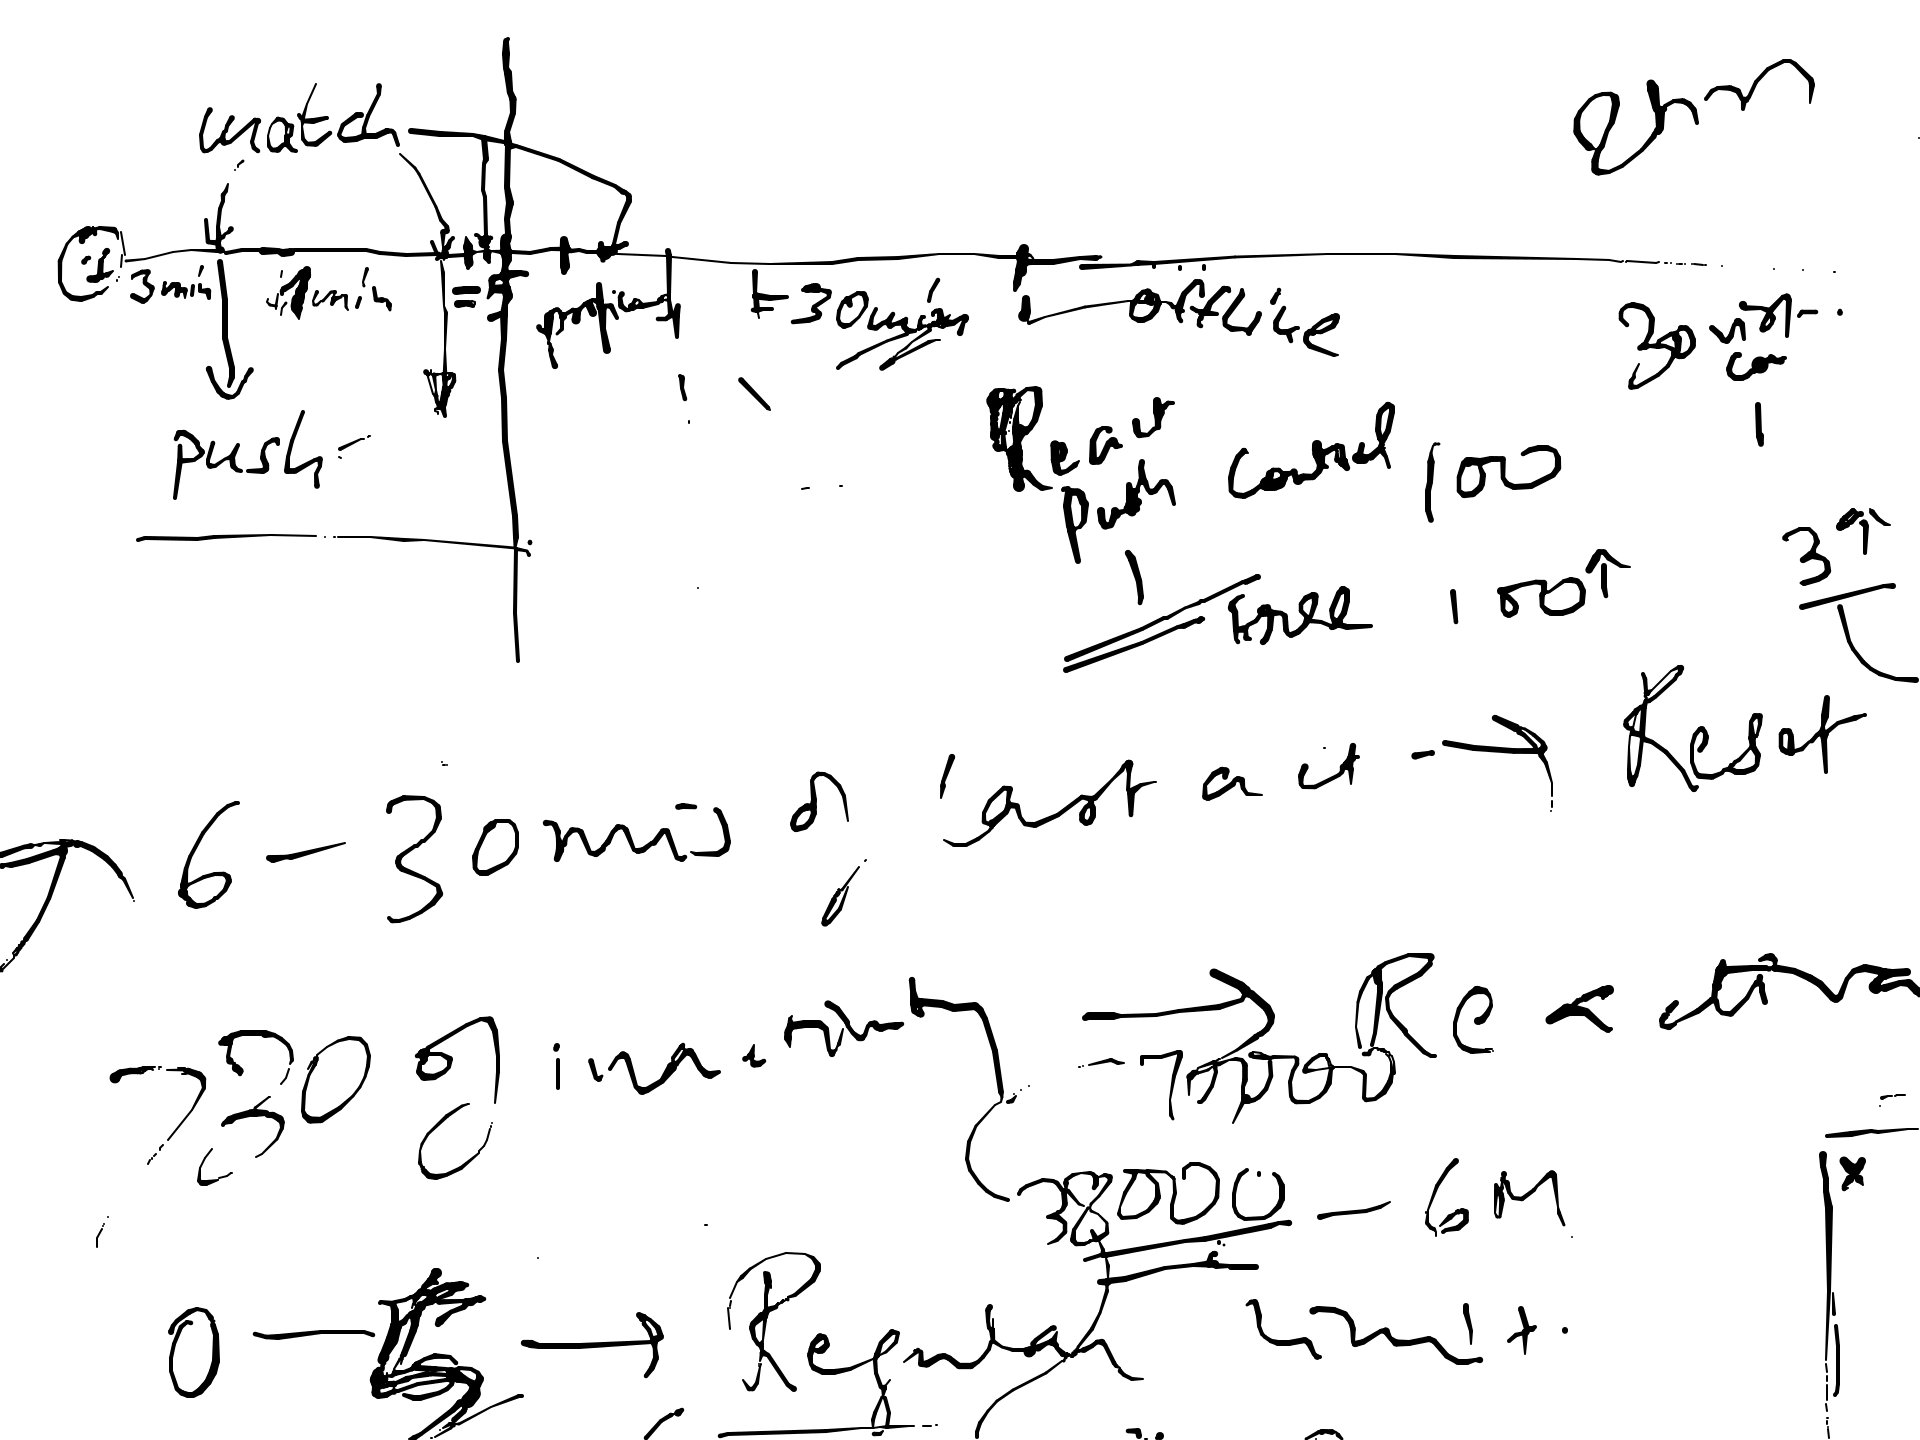
\includegraphics[width=\textwidth]{images/results_case_complex}
    \end{subfigure}

    \begin{subfigure}[t]{0.8\textwidth}
        \includesvg[inkscapelatex=false,inkscapearea=nocrop,width=\textwidth]{images/results_case_complex}
    \end{subfigure}
    \caption{Vektorisierung eines Testbilds mit hoher Komplexität (\(4032\text{px}\times3024\text{px}\))}%
    \label{fig:results_case_complex}
\end{figure}

\clearpage
\begin{listing}[htbp]
    \inputminted{cpp}{mainmatter_essentials_distance_transform_brute_force.cpp}
    \caption{Brute-Force Berechnung der exakten Euklidischen Distanztransformation}%
    \label{lst:essentials_distance_transform_brute_force}
\end{listing}

\clearpage
\begin{listing}[htbp]
    \inputminted{cpp}{mainmatter_implementation_sauvola_baseline.cpp}
    \caption[Implementation von Sauvola's Binarisierungsalgorithmus durch OpenCV]{Implementation von Sauvola's Binarisierungsalgorithmus durch OpenCV~\cite[\texttt{modules/ximgproc/src/thinning.cpp}]{opencv_contrib_source} (auf das wesentliche Reduziert)}%
    \label{lst:implementation_sauvola_baseline}
\end{listing}

\clearpage
\begin{listing}[htbp]
    \inputminted{cpp}{mainmatter_implementation_sauvola_optimized.cpp}
    \caption{Optimitierte Implementation von Sauvola's Binarisierungsalgorithmus}%
    \label{lst:implementation_sauvola_optimized}
\end{listing}

\renewcommand*\chapterpagestyle{empty}
\chapter*{Erklärung über die eigenständige Erstellung der Arbeit}

Hiermit erkläre ich, dass ich die vorgelegte Arbeit mit dem Titel

\begin{center}
	\bfseries
	Vektorisierung von Freihandzeichnungen
\end{center}

selbständig verfasst, keine anderen als die angegebenen Quellen und Hilfsmittel benutzt sowie alle wörtlich oder sinngemäß übernommenen Stellen in der Arbeit als solche und durch Angabe der Quelle gekennzeichnet habe.
Dies gilt auch für Zeichnungen, Skizzen, bildliche Darstellungen sowie für Quellen aus dem Internet.

Mir ist bewusst, dass die Hochschule für Technik und Wirtschaft Dresden Prüfungsarbeiten stichprobenartig mittels der Verwendung von Software zur Erkennung von Plagiaten überprüft.

\vspace{2cm}
\begin{tabu}{X[3]X[1]X[3]}
	Dresden, 24.04.2019 & & \\[-8bp]
	\hrulefill{} & & \hrulefill{} \\
	Ort, Datum & & Unterschrift Student
\end{tabu}


\end{document}
